\chapter{Simulação}
\label{chap:simulation}
Nessa seção, busca-se validar a abordagem integrada de Modelagem por meio de Redes de Petri Coloridas (RPC) e Controle Cooperativo. Para realizar essa validação, optou-se por empregar a estratégia de simulação, utilizando um sistema multiagente composto por diversos componentes, os quais foram concebidos para representar um ambiente similar a um sistema industrial.

Neste processo de simulação, são utilizadas ferramentas de software dedicadas à modelagem em RPC, com destaque para o CPN-Tools.\footnote{pode ser acessada em \texttt{https://cpntools.org/}} Essa ferramenta oferece funcionalidades específicas para a edição, simulação e análise de Redes de Petri Coloridas. A escolha do CPN-Tools visa proporcionar uma representação fiel e detalhada do sistema em estudo.

Para a implementação do algoritmo matemático de consenso, optou-se por utilizar a linguagem de programação Python. Essa escolha deve-se à reputação da linguagem como sendo de alto nível, funcional e orientada a objetos, oferecendo assim uma abordagem versátil e eficiente para a execução do algoritmo em questão.

Ao unir a simulação do sistema multiagente com as capacidades do CPN-Tools e a flexibilidade do Python, almeja-se obter resultados robustos que validem a eficácia da abordagem proposta. Esta seção detalhará o processo de simulação, desde a definição dos parâmetros até a análise crítica dos resultados obtidos, proporcionando uma compreensão clara e abrangente da validade e desempenho da abordagem integrada.

\section{Planta Industrial}
A gestão de vagões em uma planta industrial, que permite a ultrapassagem entre eles por meio de mudanças nas pistas, representa uma abordagem inovadora no contexto ferroviário industrial. Esse sistema dinâmico busca otimizar o movimento e a alocação de vagões, proporcionando flexibilidade e eficiência operacional.

Ao incorporar a capacidade de ultrapassagem, a planta industrial adquire versatilidade, possibilitando a reorganização estratégica dos vagões para atender a demandas específicas. Essa funcionalidade torna-se particularmente valiosa em situações onde é necessário priorizar determinados vagões, reduzir tempos de espera ou melhorar o desempenho global do sistema ferroviário dentro do contexto da planta industrial.

A implementação de mudanças nas pistas como um meio de permitir a ultrapassagem requer uma coordenação precisa e um controle eficaz do sistema. Técnicas como Redes de Petri Coloridas (RPC) ou algoritmos de controle cooperativo podem ser empregados para modelar e simular o comportamento dinâmico da planta, considerando as interações entre os vagões e as mudanças nas pistas.

Um exemplo de representação desse sistema escolhido é demonstrada na figura \ref{fig:pista_com_dois_agentes}, tal que:
\begin{itemize}
    \item Os componentes $L_1$ e $L_2$ ilustrados em formato triangular são os vagões que representam os dois autômatos, ou agentes do sistema.
    \item As curvas $d_1,d_2,..,d_6$ representam as pistas pelas quais os vagões se locomovem, de modo os dois vagões estão posicionados incialmente na pista denominada de $d_1$.
    \item os elementos $x_1,x_2,x_3,x_4$ representam as quatro chaves responsáveis por fazer a mudança de via, elas podem comutar em duas posições diferentes a posição $b$ que representa o caminho de menor comprimento ou a posição $a$ que representa o caminho de maior comprimento.
\end{itemize}

\begin{figure}[h]
\centering
\caption{Planta com pista, vagões e pontos de mudança de via }
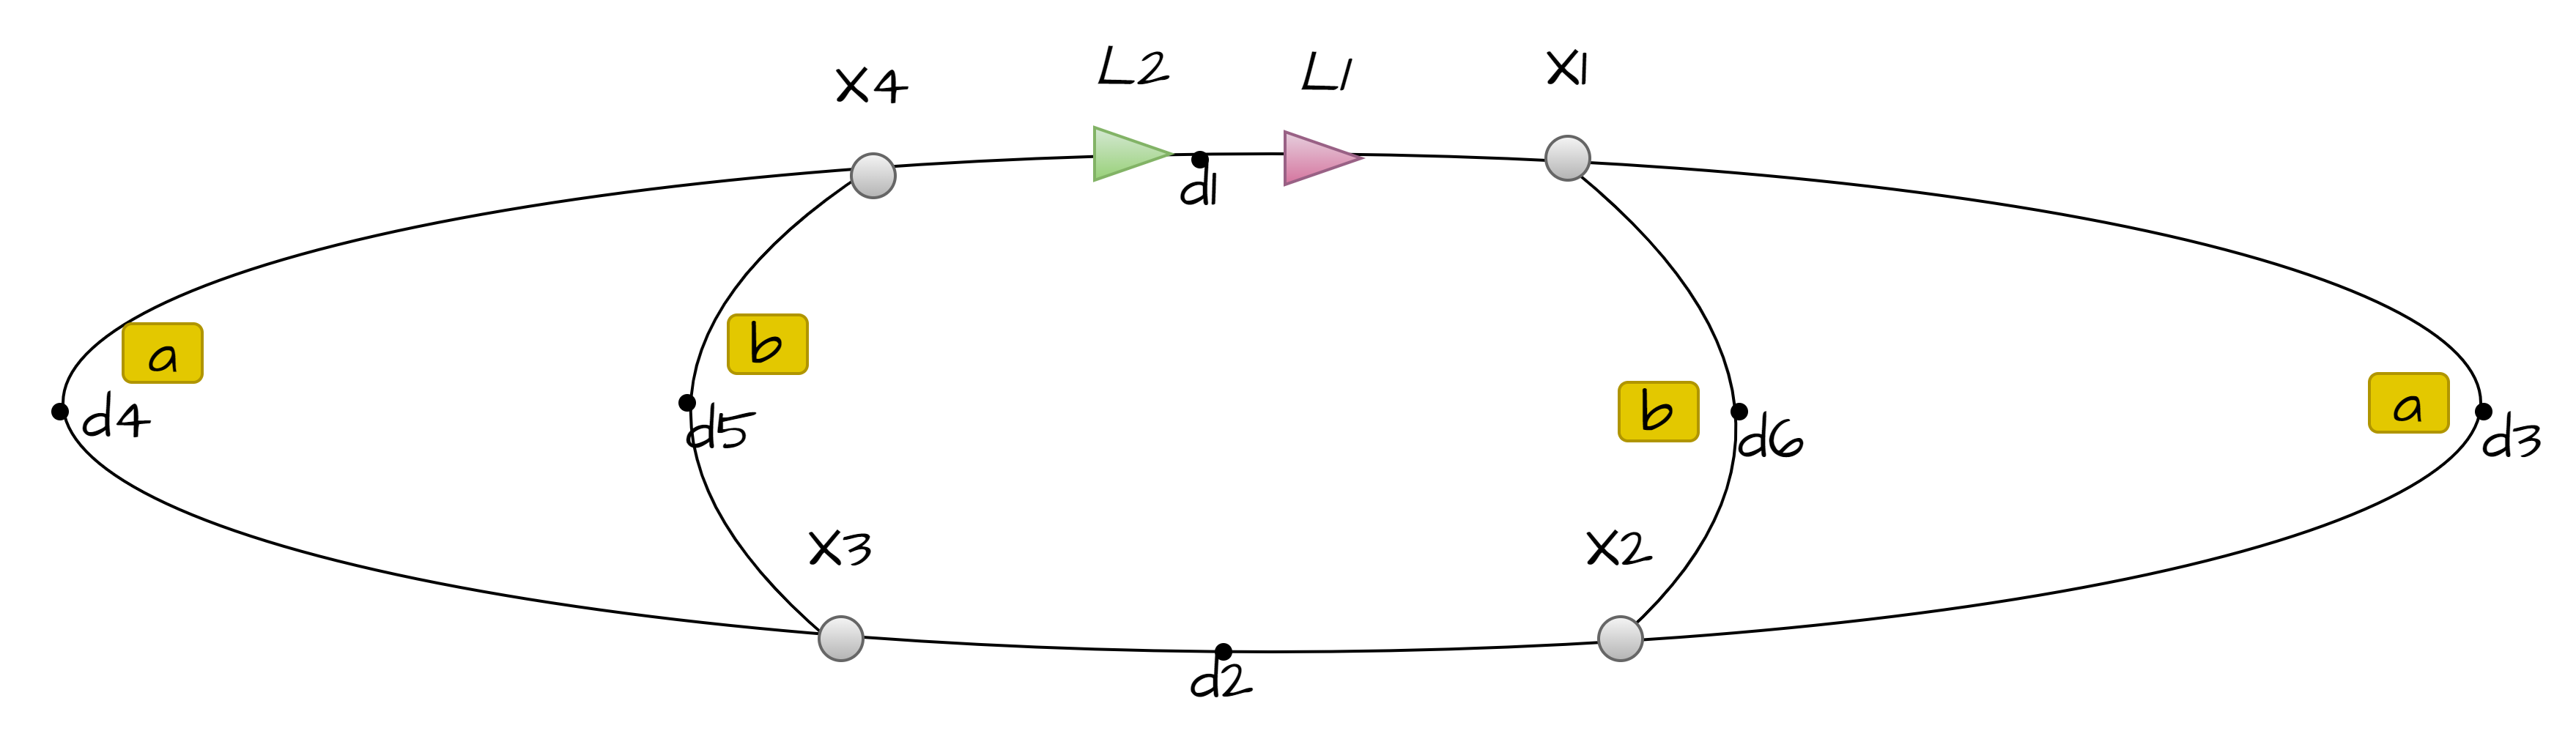
\includegraphics[width=1\linewidth]{figures/Simulation/Planta/planta_dois_agentes.png}
\label{fig:pista_com_dois_agentes}
\legend{Fonte: Elaborado pelo autor.}
\end{figure}

Para a simulação específica, os vagões movem-se entre pistas, e para efetuar uma ultrapassagem, é necessário que o vagão a ser ultrapassado siga pelo caminho mais longo, enquanto o vagão ultrapassante escolhe o caminho mais curto.

A chave de ultrapassagem foi designada como $x_1$. Quando o comando de ultrapassagem é acionado, inicialmente a chave se move para a posição $a$, assegurando o desvio para a pista mais longa. Em seguida, ela se move para a posição $b$, garantindo o desvio para a pista mais curta.

A chave $x_2$ desempenha o papel de primeiro desviar para a posição $b$, para receber o vagão da pista $d_6$. Posteriormente, comuta para a posição $a$, para receber o vagão da pista $d_3$.

As chaves $x_3$ e $x_4$ permanecem fixas na posição $b$, assegurando o percurso mais curto. Esse arranjo permite uma ultrapassagem de vagões de forma segura e otimizada entre as pistas.

\section{Modelagem em Redes de Petri Colorida}
\label{sec:model_RPC}
Para a modelagem do sistema proposto em Redes de Petri Colorida, foi definido o seguinte conjunto de cores para representar o tipo de token que vai ser alocado nos lugares da RPC de acordo com o seguinte quadro \ref{qua:conj_cores}.

\begin{quadro}[h]
\centering
\caption{Conjunto de Cores na RPC}
\begin{tabularx}{\textwidth}{|c|c|X|X|}
\hline
\textbf{Nomenclatura} & \textbf{Tipo}    & \textbf{Comando}                             & \textbf{Descrição} \\
\cline{1-4}
D & Inteiro & \texttt{colset D = int;} 
& Conjunto que indica a sequência dos vagões, onde o número 1 representa o vagão à frente, o número 2 representa o vagão atrás do 1, e assim por diante. \\ 
\cline{1-4}
X & String  & \texttt{colset X = string;} 
& Conjunto que representa a posição em que a chave se encontra, exemplo "a" para a posição A e "b" para a posição B. \\
\cline{1-4}
L & String  & \texttt{colset L = string;}         
& Conjunto de cores que representa os vagões ao longo da pista em que "L\_1" é o vagão L1 e "L\_2" o vagão L2. \\
\cline{1-4}
Ord & Record  & \texttt{colset Ord = record seq:D * train:L;} 
& Conjunto de cores que representa a associação do vagão L com a posição D,
de modo que caso "L1" esteja na primeira posição, será representado por "seq:1,train:L1". \\ 
\cline{1-4}

\end{tabularx}
\legend{Fonte: Elaborado pelo autor.}
\label{qua:conj_cores}
\end{quadro}

 Para cada conjunto de cores foi definido as variáveis correspondentes que serão alocados na inscrição dos arcos ao longo da RPC, de acordo com o quadro \ref{qua:variaveis_RPC}.

\begin{quadro}[ht]
\caption{Conjunto de Variáveis na RPC}
\begin{tabularx}{\textwidth}{|c|c|c|X|}
\cline{1-4}
% Cabeçalho
\textbf{Variável} & \textbf{Tipo} & \textbf{Exemplo} & \textbf{Descrição} \\ 
\cline{1-4} % Linha 1
d & D & 1`(1) ou 1`(2) & Variável de tipo Inteira, no exemplo tem-se 1 ficha com o valor 1, ou 2 fichas com valor 1, mais uma ficha com valor 2 \\ \cline{1-4} % Linha 2
x & X & 1`("a") ou 1`("b") & Variável do Tipo \textit{String} referente a posição de chave, pode ser do tipo "a" ou do tipo "b",como no exemplo. \\ \cline{1-4} % Linha 3
l & L & 1`("l1") ou 1`("l2") & Variável do Tipo \textit{String} referente ao vagão/trem que nos casos podem ser do tipo "l1" ou "l2", como no exemplo para dois agentes \\ \cline{1-4} % Linha 4
ord & Ord & 1`\{seq=2,train="l1"\} & Variável do Tipo \textit{record seq:d * train:L}, no exemplo descrito indica que o trem "l1" está na posição 2. \\ \cline{1-4} 
\end{tabularx}
\label{qua:variaveis_RPC}
\legend{Fonte:Elaborado pelo Autor}
\end{quadro}

Para a abstração e melhor organização e legibilidade da representação na RPC, foram definidos dois níveis hierárquico o nível mais acima da Pista, e o nível mais abaixo o de controle e comando. Cada nível possui um conjunto de módulos que podem ser agrupados em 3 principais funcionalidades, Pista, Controle das Chaves "X" e controle de Ordenação dos vagões "L", como demonstrado na figura \ref{fig:hierarquia_RPC}. Observa-se que para o controle das chaves X, foi definido 4 módulos de controle 1 para cada chave, que são responsáveis por gerenciar em qual posição cada respectiva chave irá estar. No caso do componente de Controle de Ordenação foram definidos 2 módulos, o de "Ordem", responsável por gerar o comando de "Ultrapassagem" ou "Não Ultrapassagem", já o módulo de "Inverter Ordem" é responsável por atualizar as ordem do vagões através da leitura da pista.

\begin{figure}[ht]
    \centering
    \caption{Modelo dos Componentes Hierárquicos da RPC}
    \label{fig:hierarquia_RPC}
    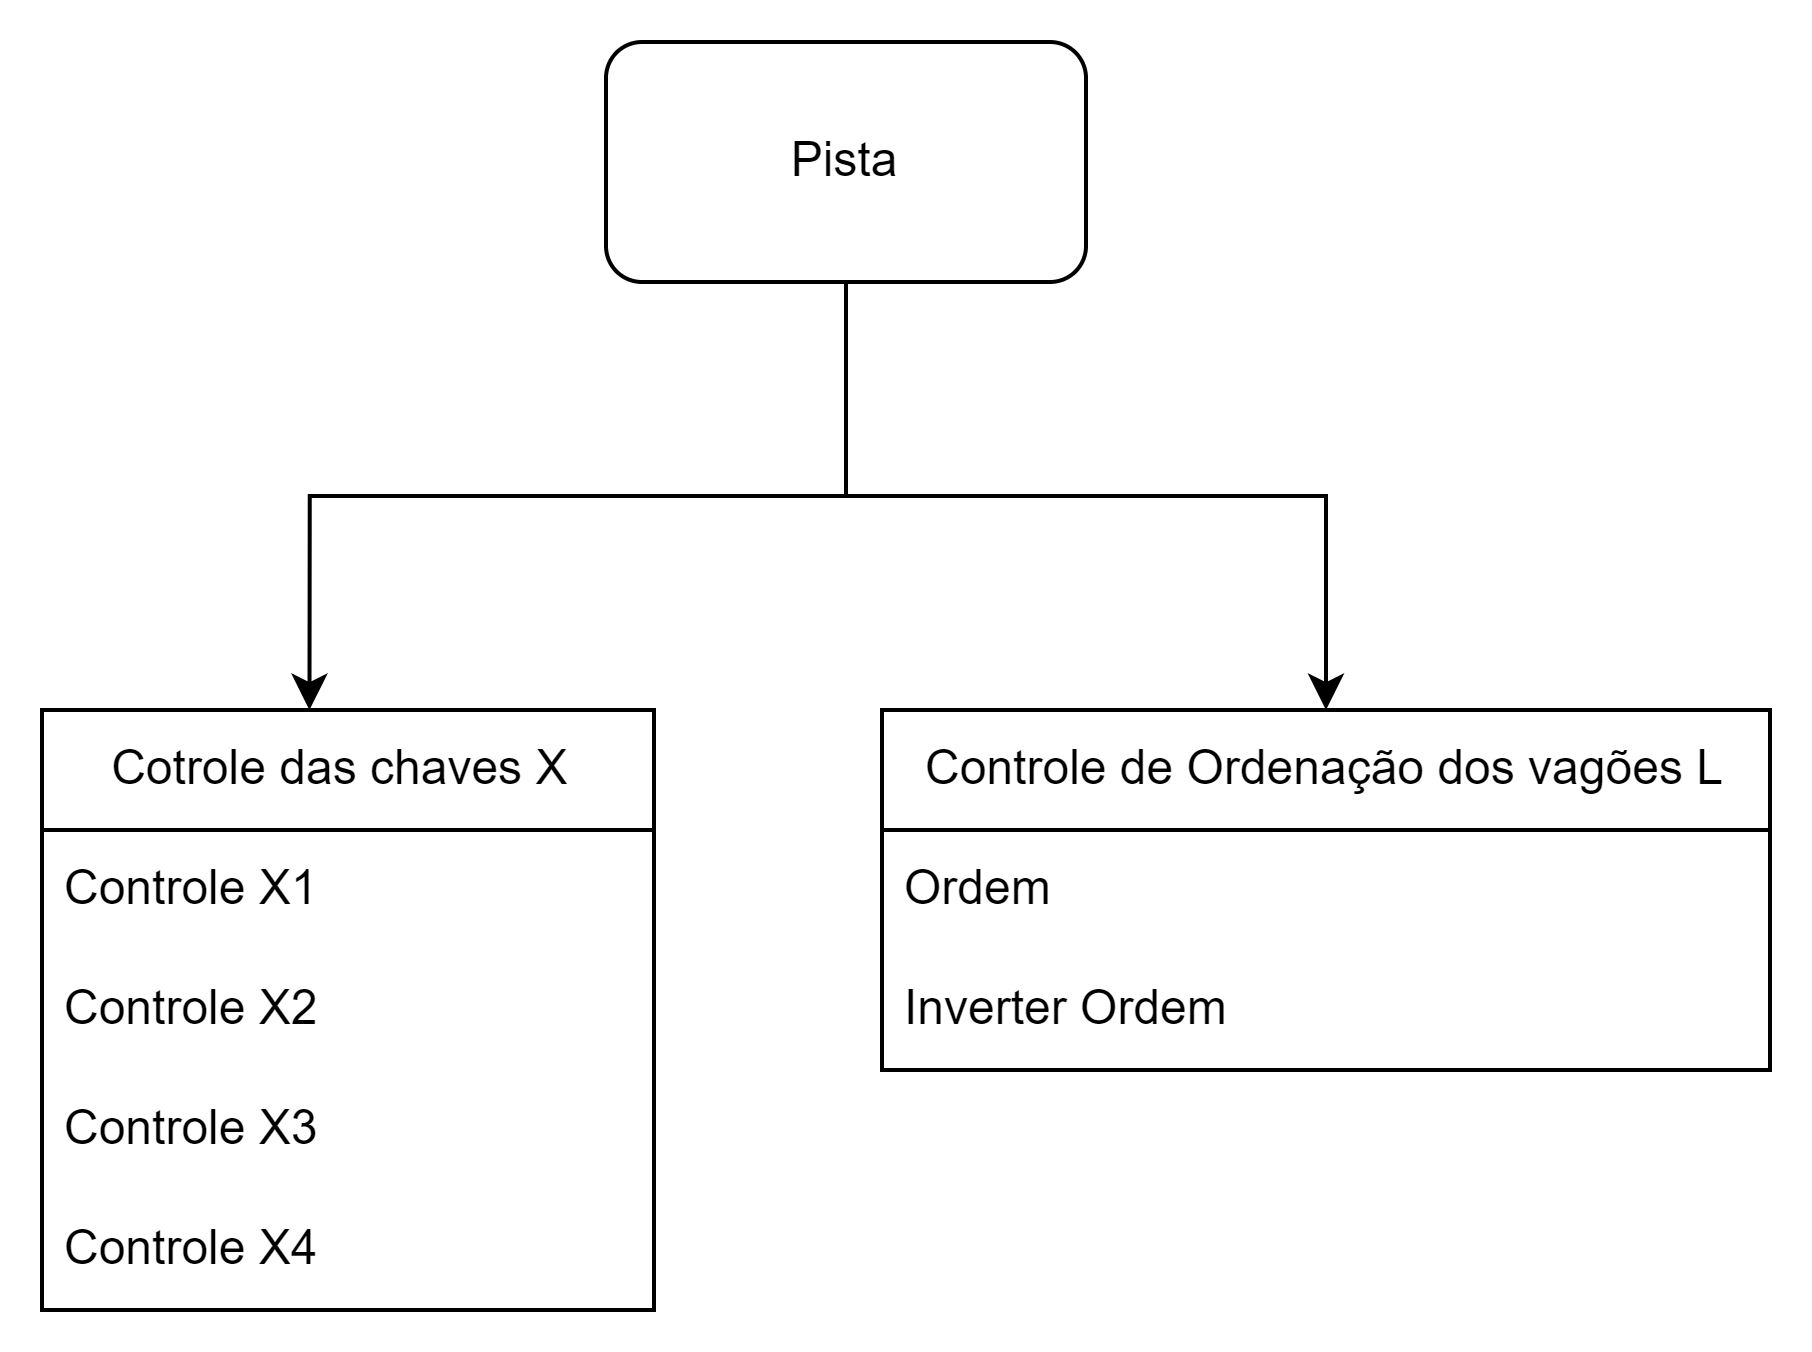
\includegraphics[width=0.8\linewidth]{figures//Simulation//Modelagem/hierarquia.png}
    \legend{Fonte: Elaborado pelo autor.}
\end{figure}

A RPC de camada superior é dada pela figura \ref{fig:rede_geral}, nela é possível verifica a existência de outras sub-redes dada pelas transições \textit{Controle} $X_1$ a $X_4$ e \textit{Ordem} e \textit{Inverter Ordem}, dadas pelas transições com dupla bordas, que correpondem aos componentes de mais baixa hierarquia modelado através da figura \ref{fig:hierarquia_RPC}.

\begin{figure}[ht]
    \centering
    \caption{Rede de Nível Hierárquico superior}
    \label{fig:rede_geral}
    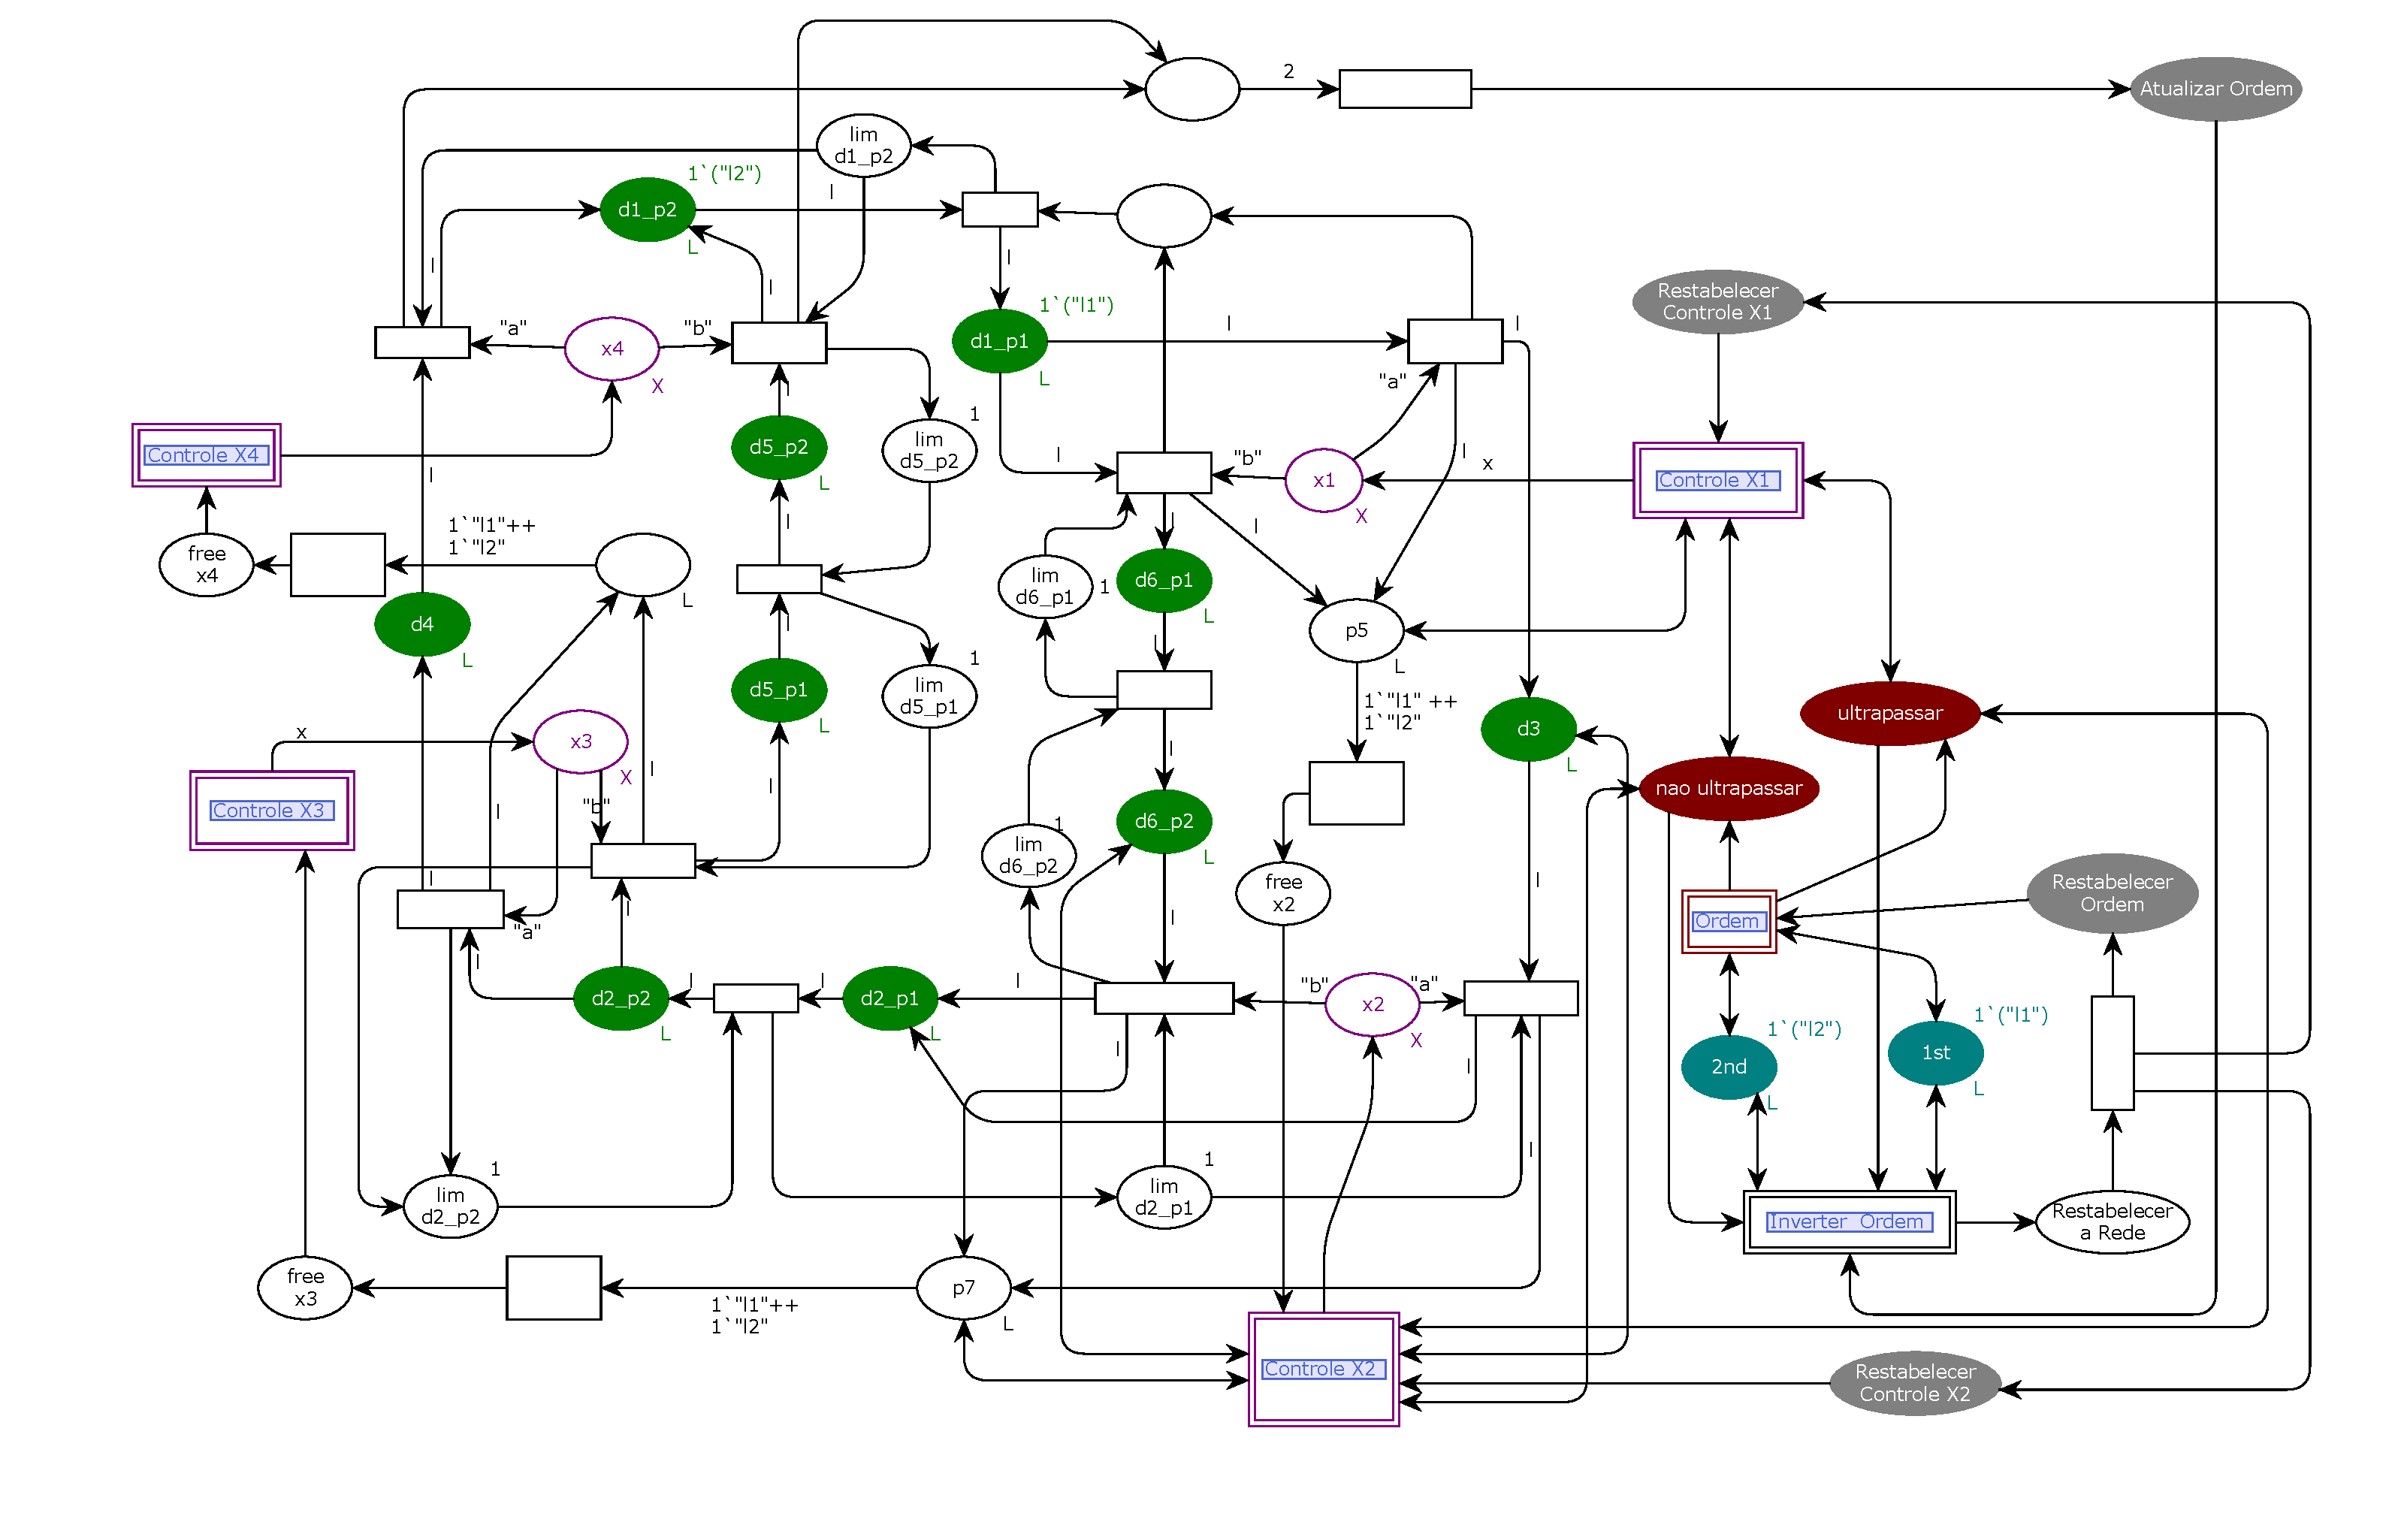
\includegraphics[width=1\linewidth]{figures/Simulation/Modelagem/rede_geral.eps}
    \legend{Fonte: Elaborado pelo autor.}
\end{figure}


\subsection{Modelagem da Pista}
\label{sub:model_pista}
A modelagem da pista foi feito através do conjunto de lugares e transições que representam o movimento e mecanismos pelos quais os vagões iram transitar, a modelagem completa dada pela figura \ref{fig:rede_geral} foi dividida em algumas máscaras (representação parcial da rede) para melhor visualização ao longo da sub seção. 

A figura \ref{fig:pista_RPC} demonstra os principais componentes das pista, tal que os lugares de $d_1$ a $d_6$ referem-se as curvas da pista representada na figura \ref{fig:pista_com_dois_agentes}. Observe que o conjunto de cores nesses lugares são o conjunto $L$, indicando que neles transitam as fichas do tipo vagões que podem ser "$l_1$" ou "$l_2$" como nos casos do lugar $d_1\_p_1$ e $d_1\_p_2$ respectivamente. Assim de modo análogo os arcos que referentes a movimentação das fichas do tipo \textit{L} são da variável tipo \textit{l} que controla os graus de saída e entrada das transições que movimentam os vagões ao longo da pista. Também é modelado os locais de junções e divisões, por exemplo no lugar $d_1\_p_1$ que representa a área $1$ da pista $d_1$ nela a pista sofre uma divisão, de modo que o vagão pode ir ou para a curva $d_6$ ou para a curva $d_3$ da pista. Os locais de junção ocorrem por exemplo na curva $d_2\_p_1$ da pista, em que recebe tanto os vagões que veem da pista $d_3$, quanto da pista $d_6$.
\begin{figure}[ht]
    \centering
    \caption{Máscara dos Componentes da pista na RPC}
    \label{fig:pista_RPC}
    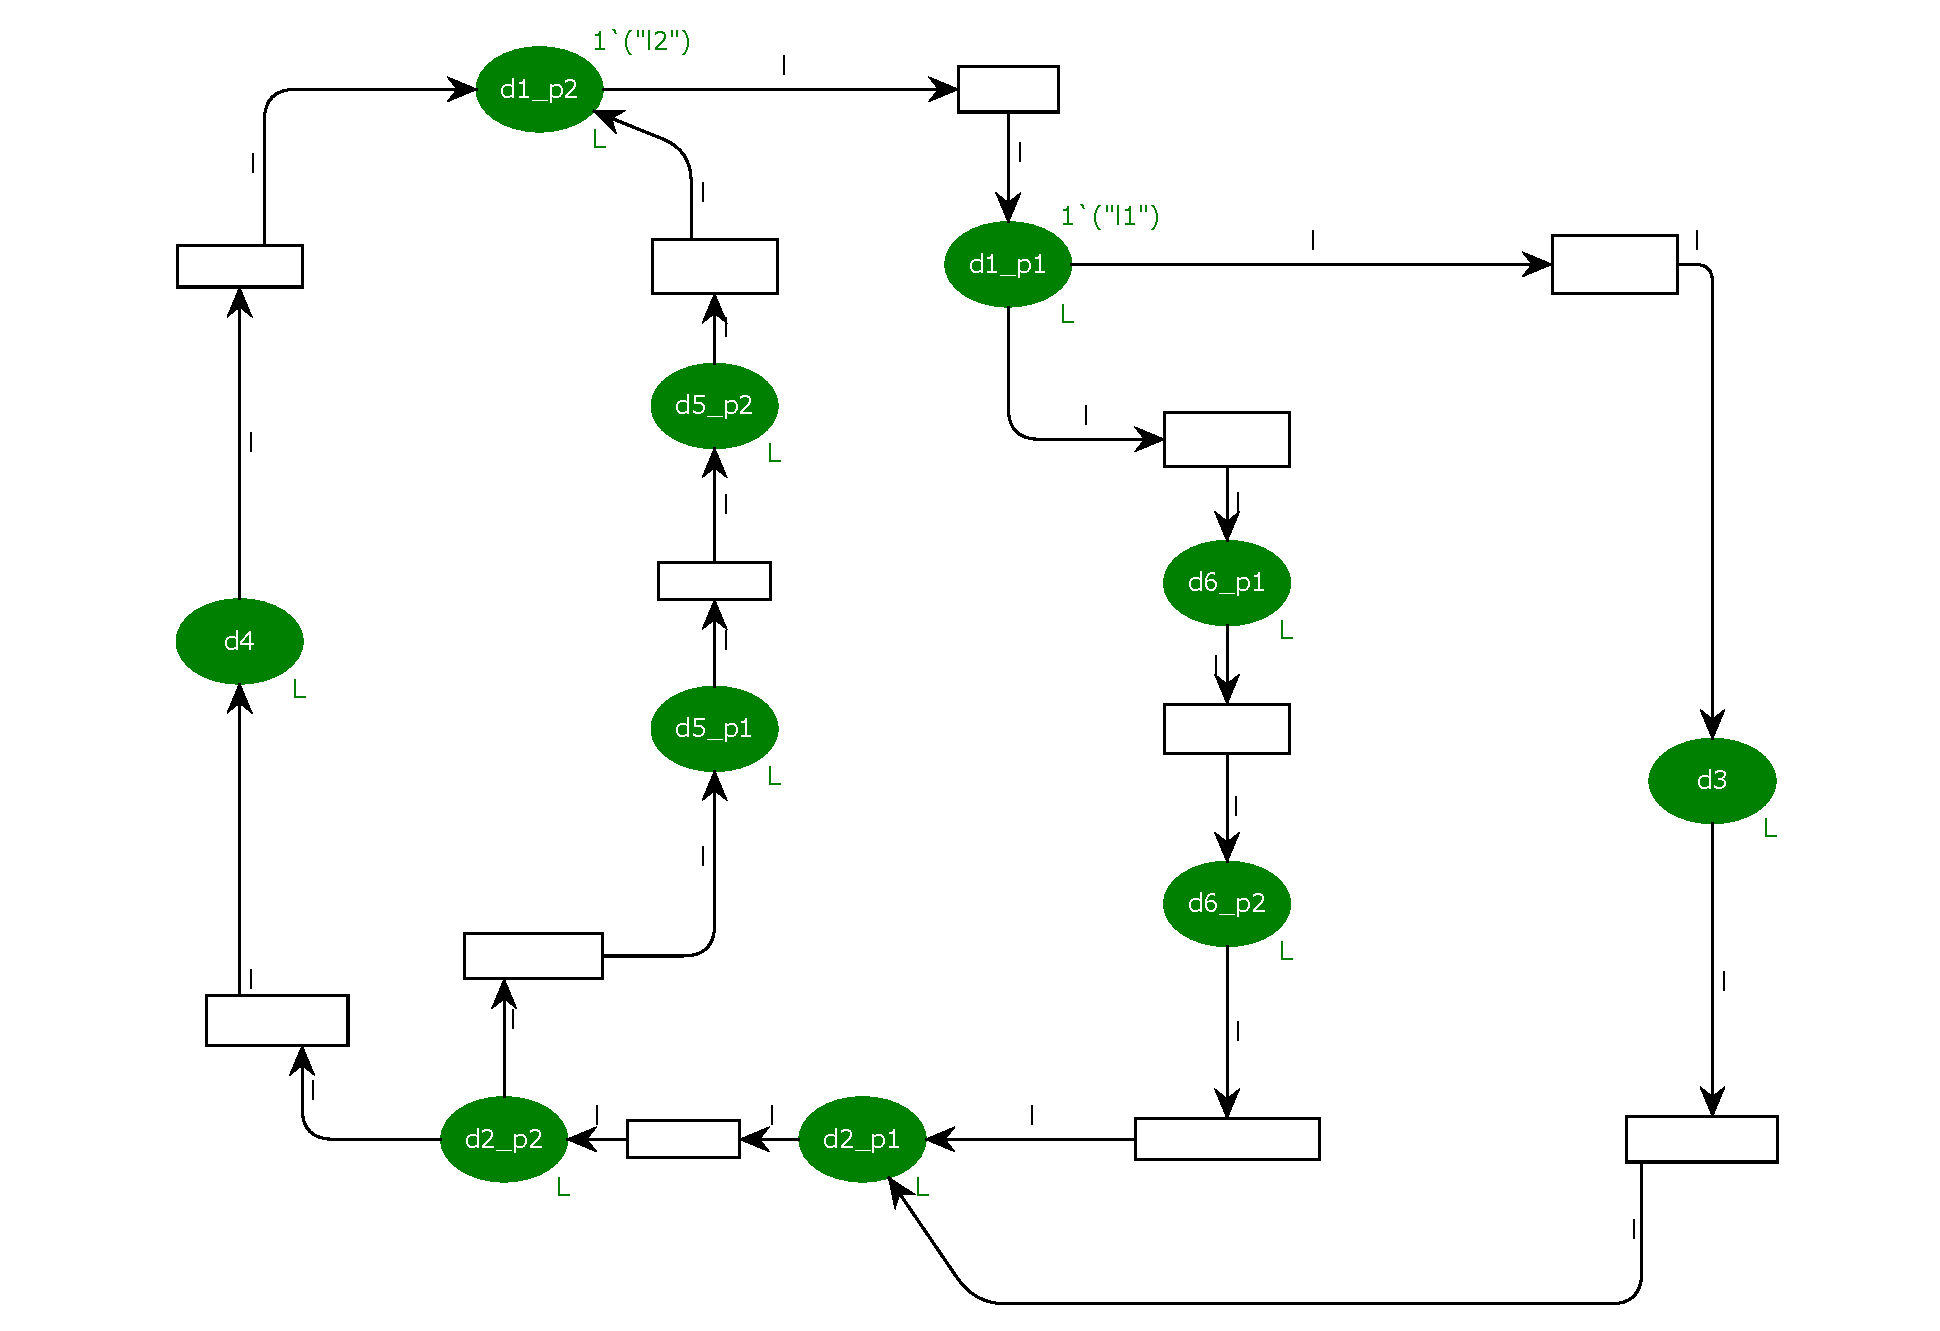
\includegraphics[width=1\linewidth]{figures//Simulation//Modelagem/pista.eps}
    \legend{Fonte: Elaborado pelo autor.}
\end{figure}

Para a modelagem da pista também é importante a implementação do conceito limitadores de região, que são lugares que controlam a quantidade de vagões por região, que para níveis de modelagem na RPC são importantes para evitar que dois vagões estejam na mesma região ao mesmo tempo. Os limitadores de região são implementados em algumas regiões como demonstrado na figura \ref{fig:limitadores_pista}, de modo que quando o vagão entra em determinada região é retirado uma ficha do lugar \textit{lim} ${d_x\_p_y}$, desabilitando a transição que permite a entrada de um vagão naquela região, tal ficha é devolvida quando o vagão que está sai para outra região. 

Por exemplo, note que para que uma ficha entre no lugar $d_5\_p_2$ é necessário que haja uma ficha no lugar \textit{lim} $d_5\_p_2$, e que ao entrar nessa região uma ficha é consumida e ao sair a ficha é retornada ao limitador garantido que somente um vagão ocupara aquela região por vez.

\begin{figure}[ht]
    \centering
    \caption{Máscara dos Componentes da pista com o controle das chaves na RPC}
    \label{fig:limitadores_pista}
    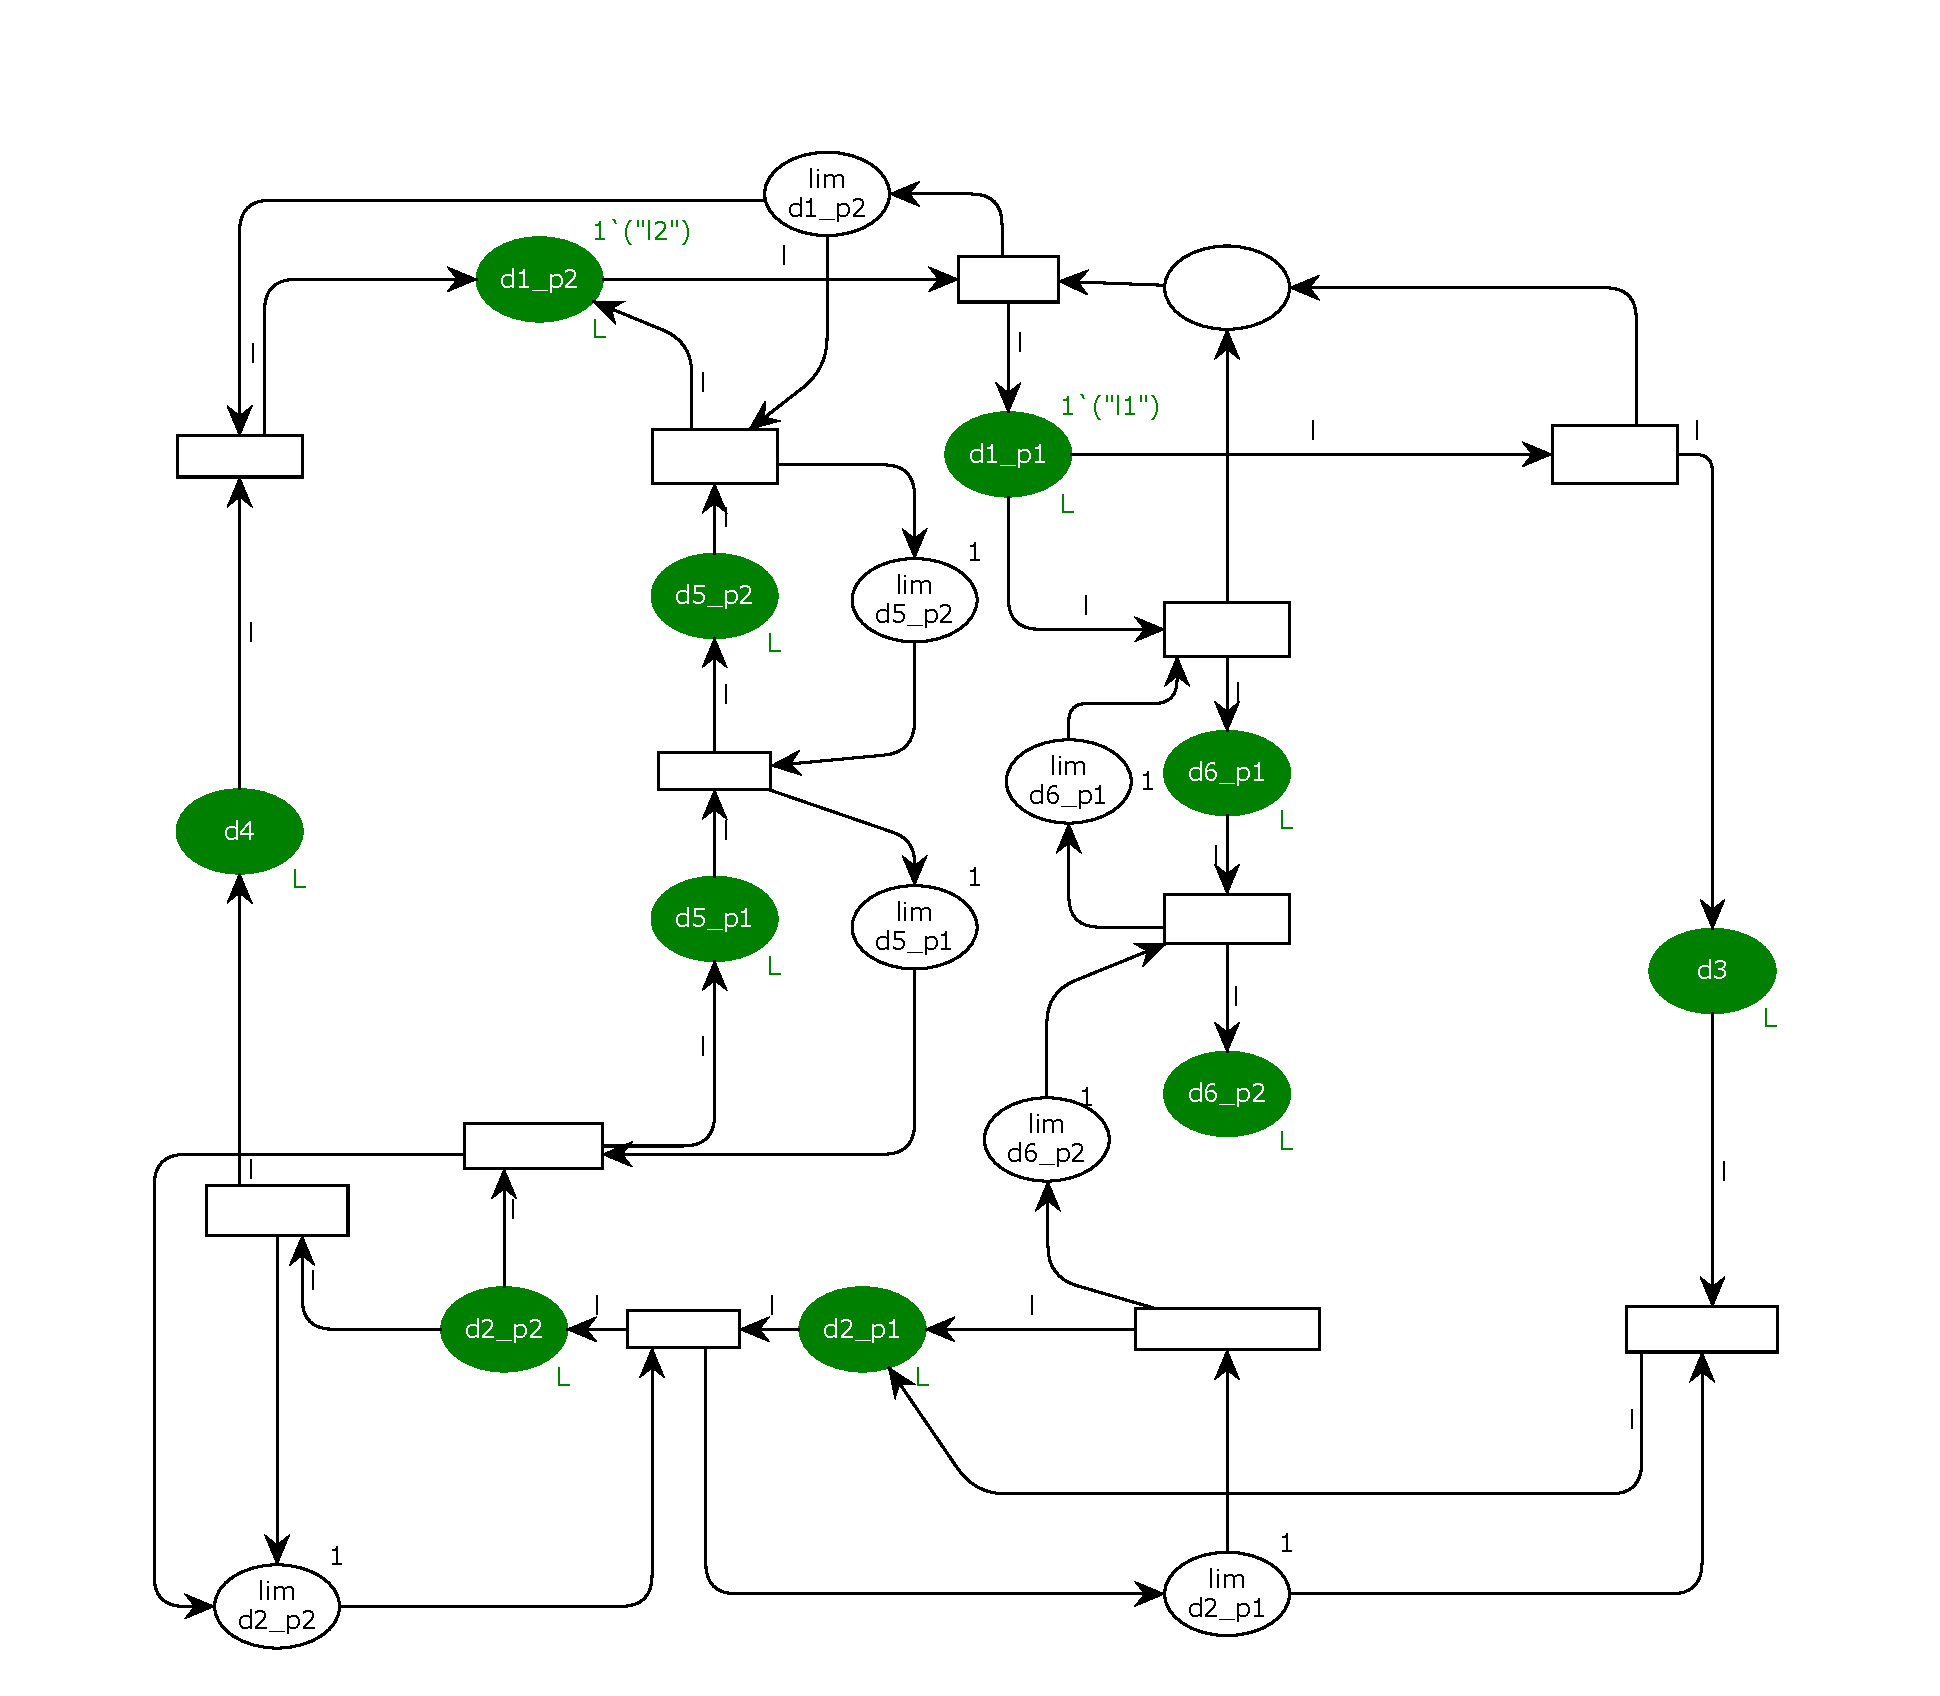
\includegraphics[width=1\linewidth]{figures//Simulation//Modelagem/limitadores_pista.eps}
    \legend{Fonte: Elaborado pelo autor.}
\end{figure}

Outro conceito fundamental na modelagem de uma RPC é o de reestabelecimento da rede, garantido que ao chegar no final do ciclo de uma volta a rede continue em funcionamento para um número ilimitado de iterações, tal reestabelecimento é demonstrado na figura \ref{fig:restabelecer_geral}. Note que após a segunda ativação da chave $X_4$ é dado o comando de atualizar a ordem vigente dos vagões e logo em seguida é dado o comando de \textit{Reestabelecer a Rede}, enviando a ficha para reestabelecer os \textit{Controles} $X_1 e X_2$ assim como o \textit{Controle de Ordem}.

\begin{figure}[ht]
    \centering
    \caption{Máscara dos Componentes de reestabelecimento na RPC}
    \label{fig:restabelecer_geral}
    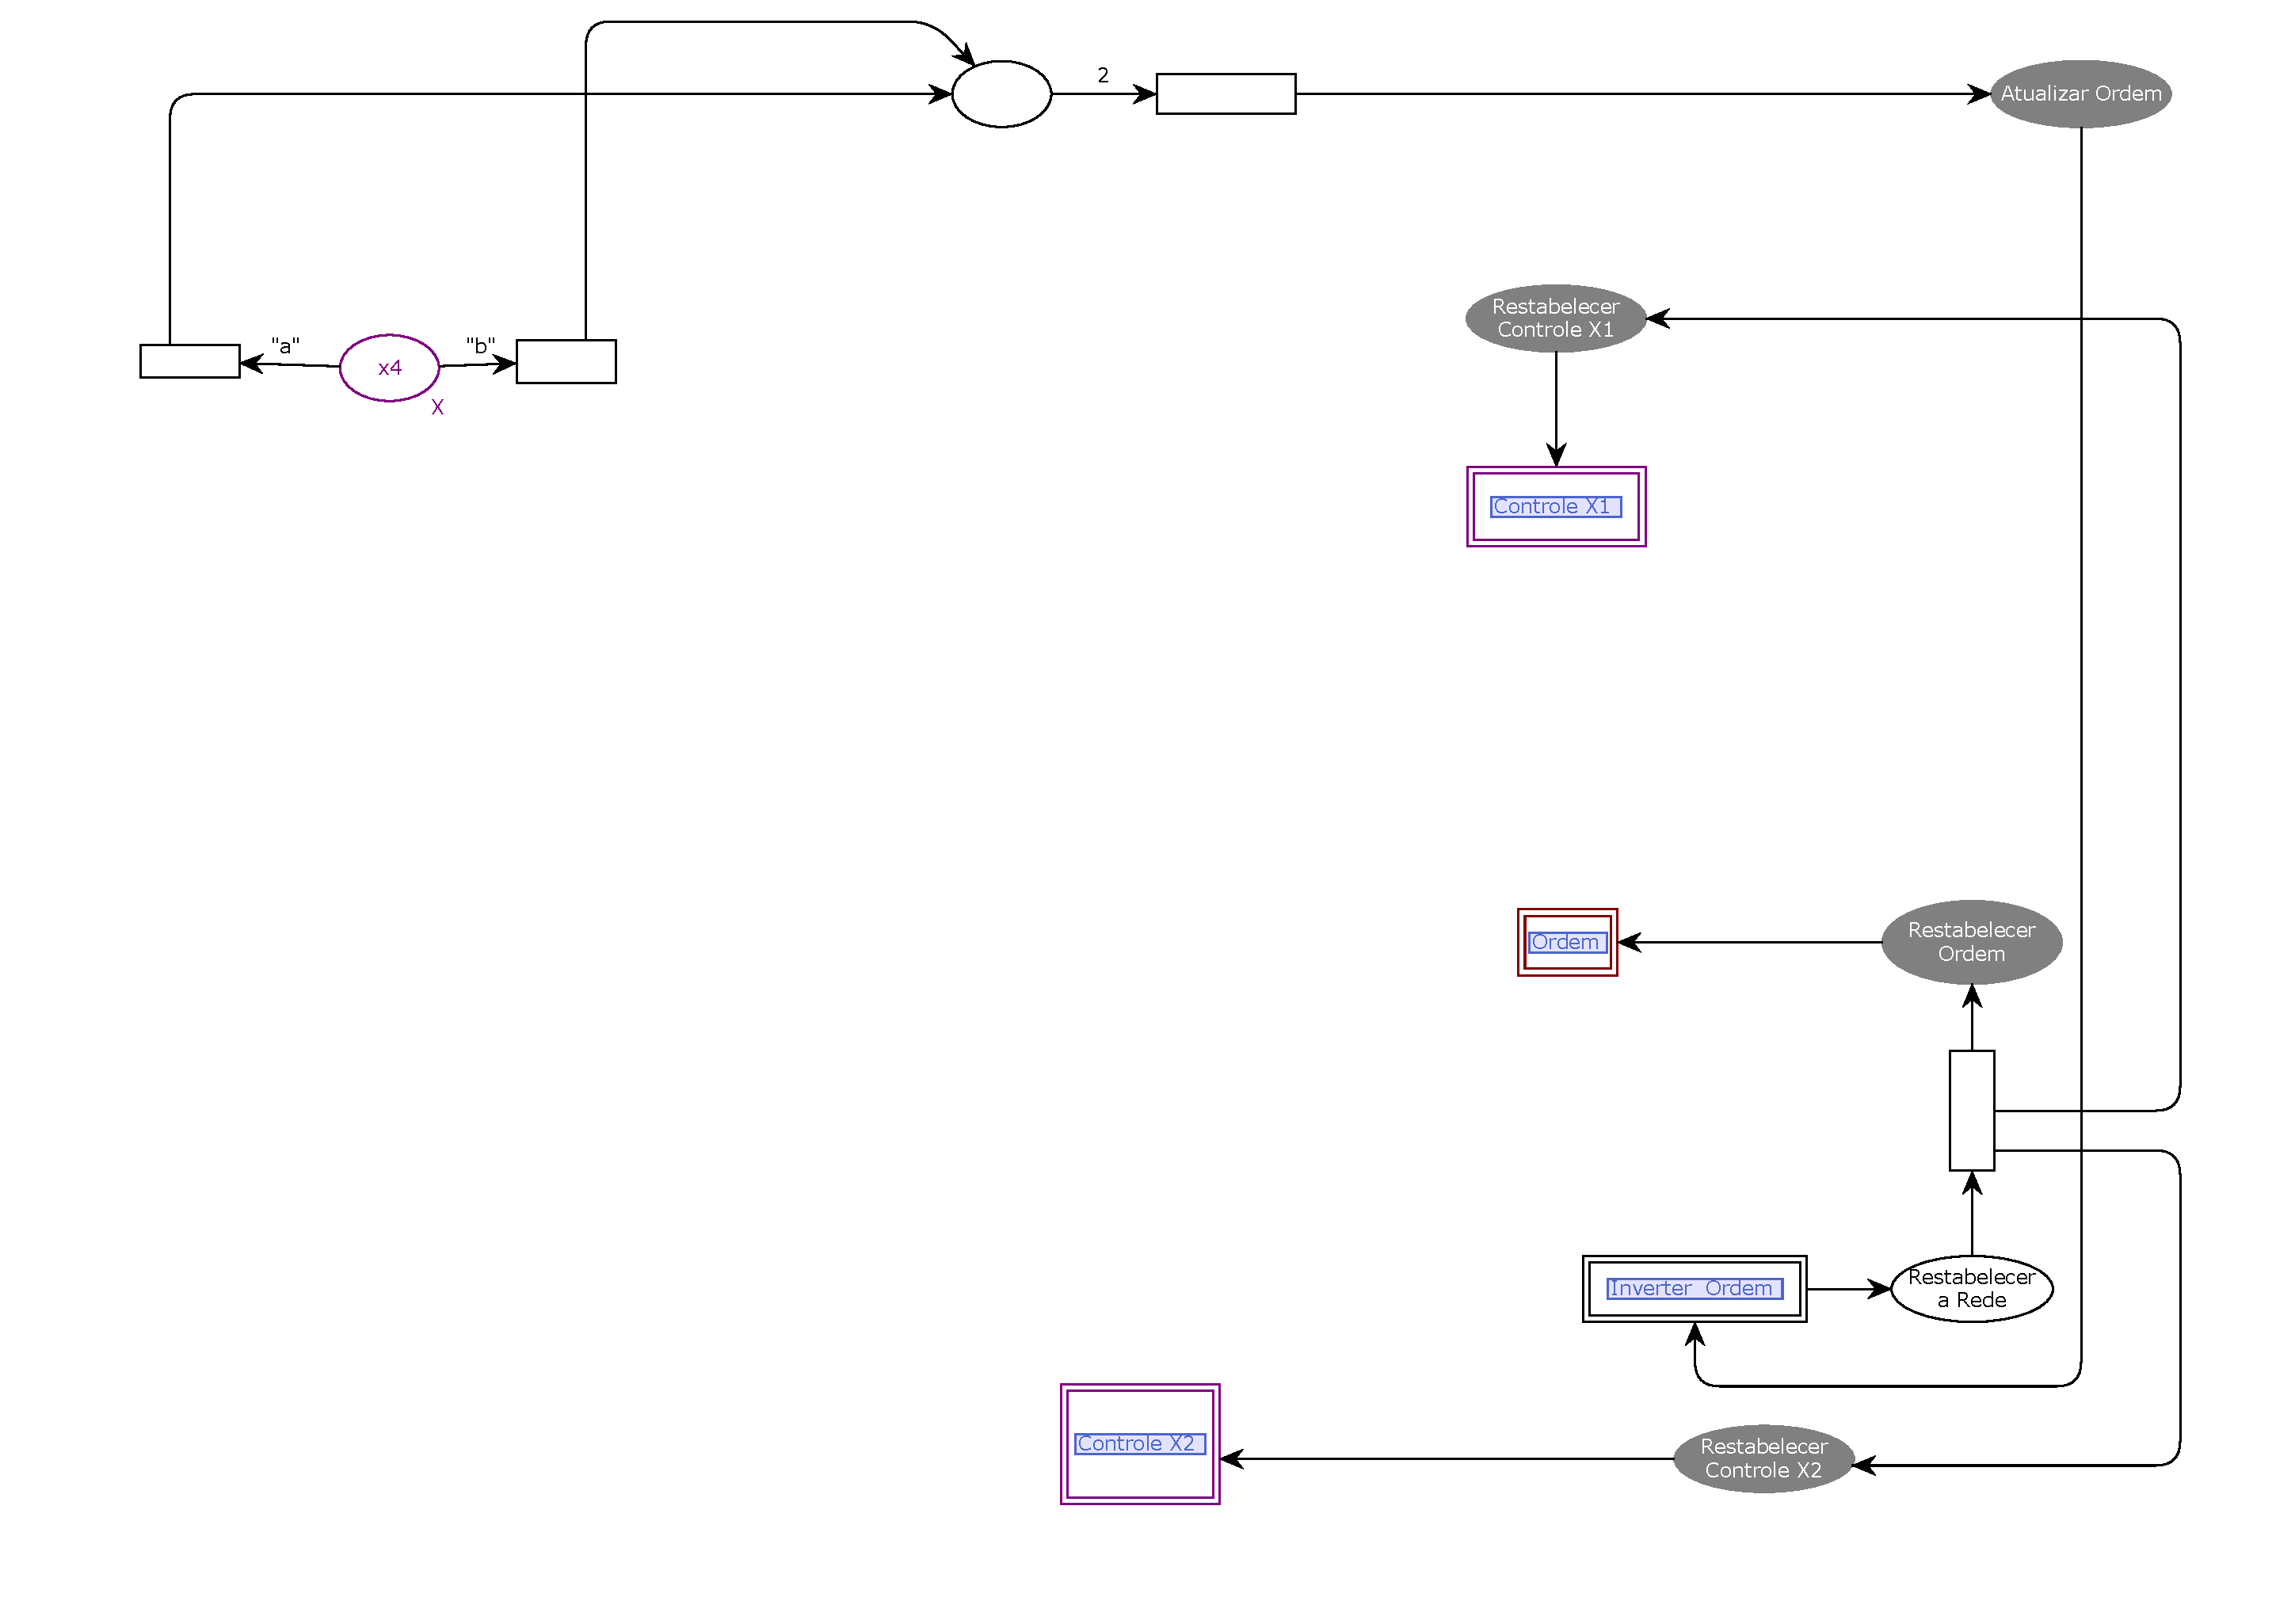
\includegraphics[width=1\linewidth]{figures/Simulation/Modelagem/restabelecer_geral.eps}
    \legend{Fonte: Elaborado pelo autor.}
\end{figure}

\clearpage
\subsection{Modelagem Controladores}
Considerando o modelo anterior na subseção \ref{sub:model_pista} de organização das pistas a figura \ref{fig:pista_chaves_RPC} representa além dos componentes fundamentas das curvas das pistas $d_1$ a $d_6$, os componentes de chaves \textit{X}, com as transições hierárquicas de \textit{Controle} $X_1$ a \textit{Controle} $X_4$. Observe que nos pontos de junção e divisão se encontroam os locais $X_1$ a $X_4$, que pertencem ao conjunto \textit{X} que podem receber fichas do tipo "a" ou "b" como explicado no quadro \ref{qua:variaveis_RPC}, tais lugares controlam as condições de acionamento das transições ligadas os arcos de saída. 

Por exemplo, dado um ficha "1`$(l_1)$" no lugar $d_1\_p_1$ quem vai definir qual transição será habilita, se para ir para a pista $d_3$ ou para a pista $d_6$, será a ficha no lugar $x_1$, que é controlada pela transição hierárquica \textit{Controle} $X_1$. Tal que dependendo da ficha que o local \textit{X} receber pelos respectivos Controladores será habilitada e desabilitada as transições que ligam as curvas ao longo da pista. 
\begin{figure}[ht]
    \centering
    \caption{Máscara dos Componentes da pista com o controle das chaves na RPC}
    \label{fig:pista_chaves_RPC}
    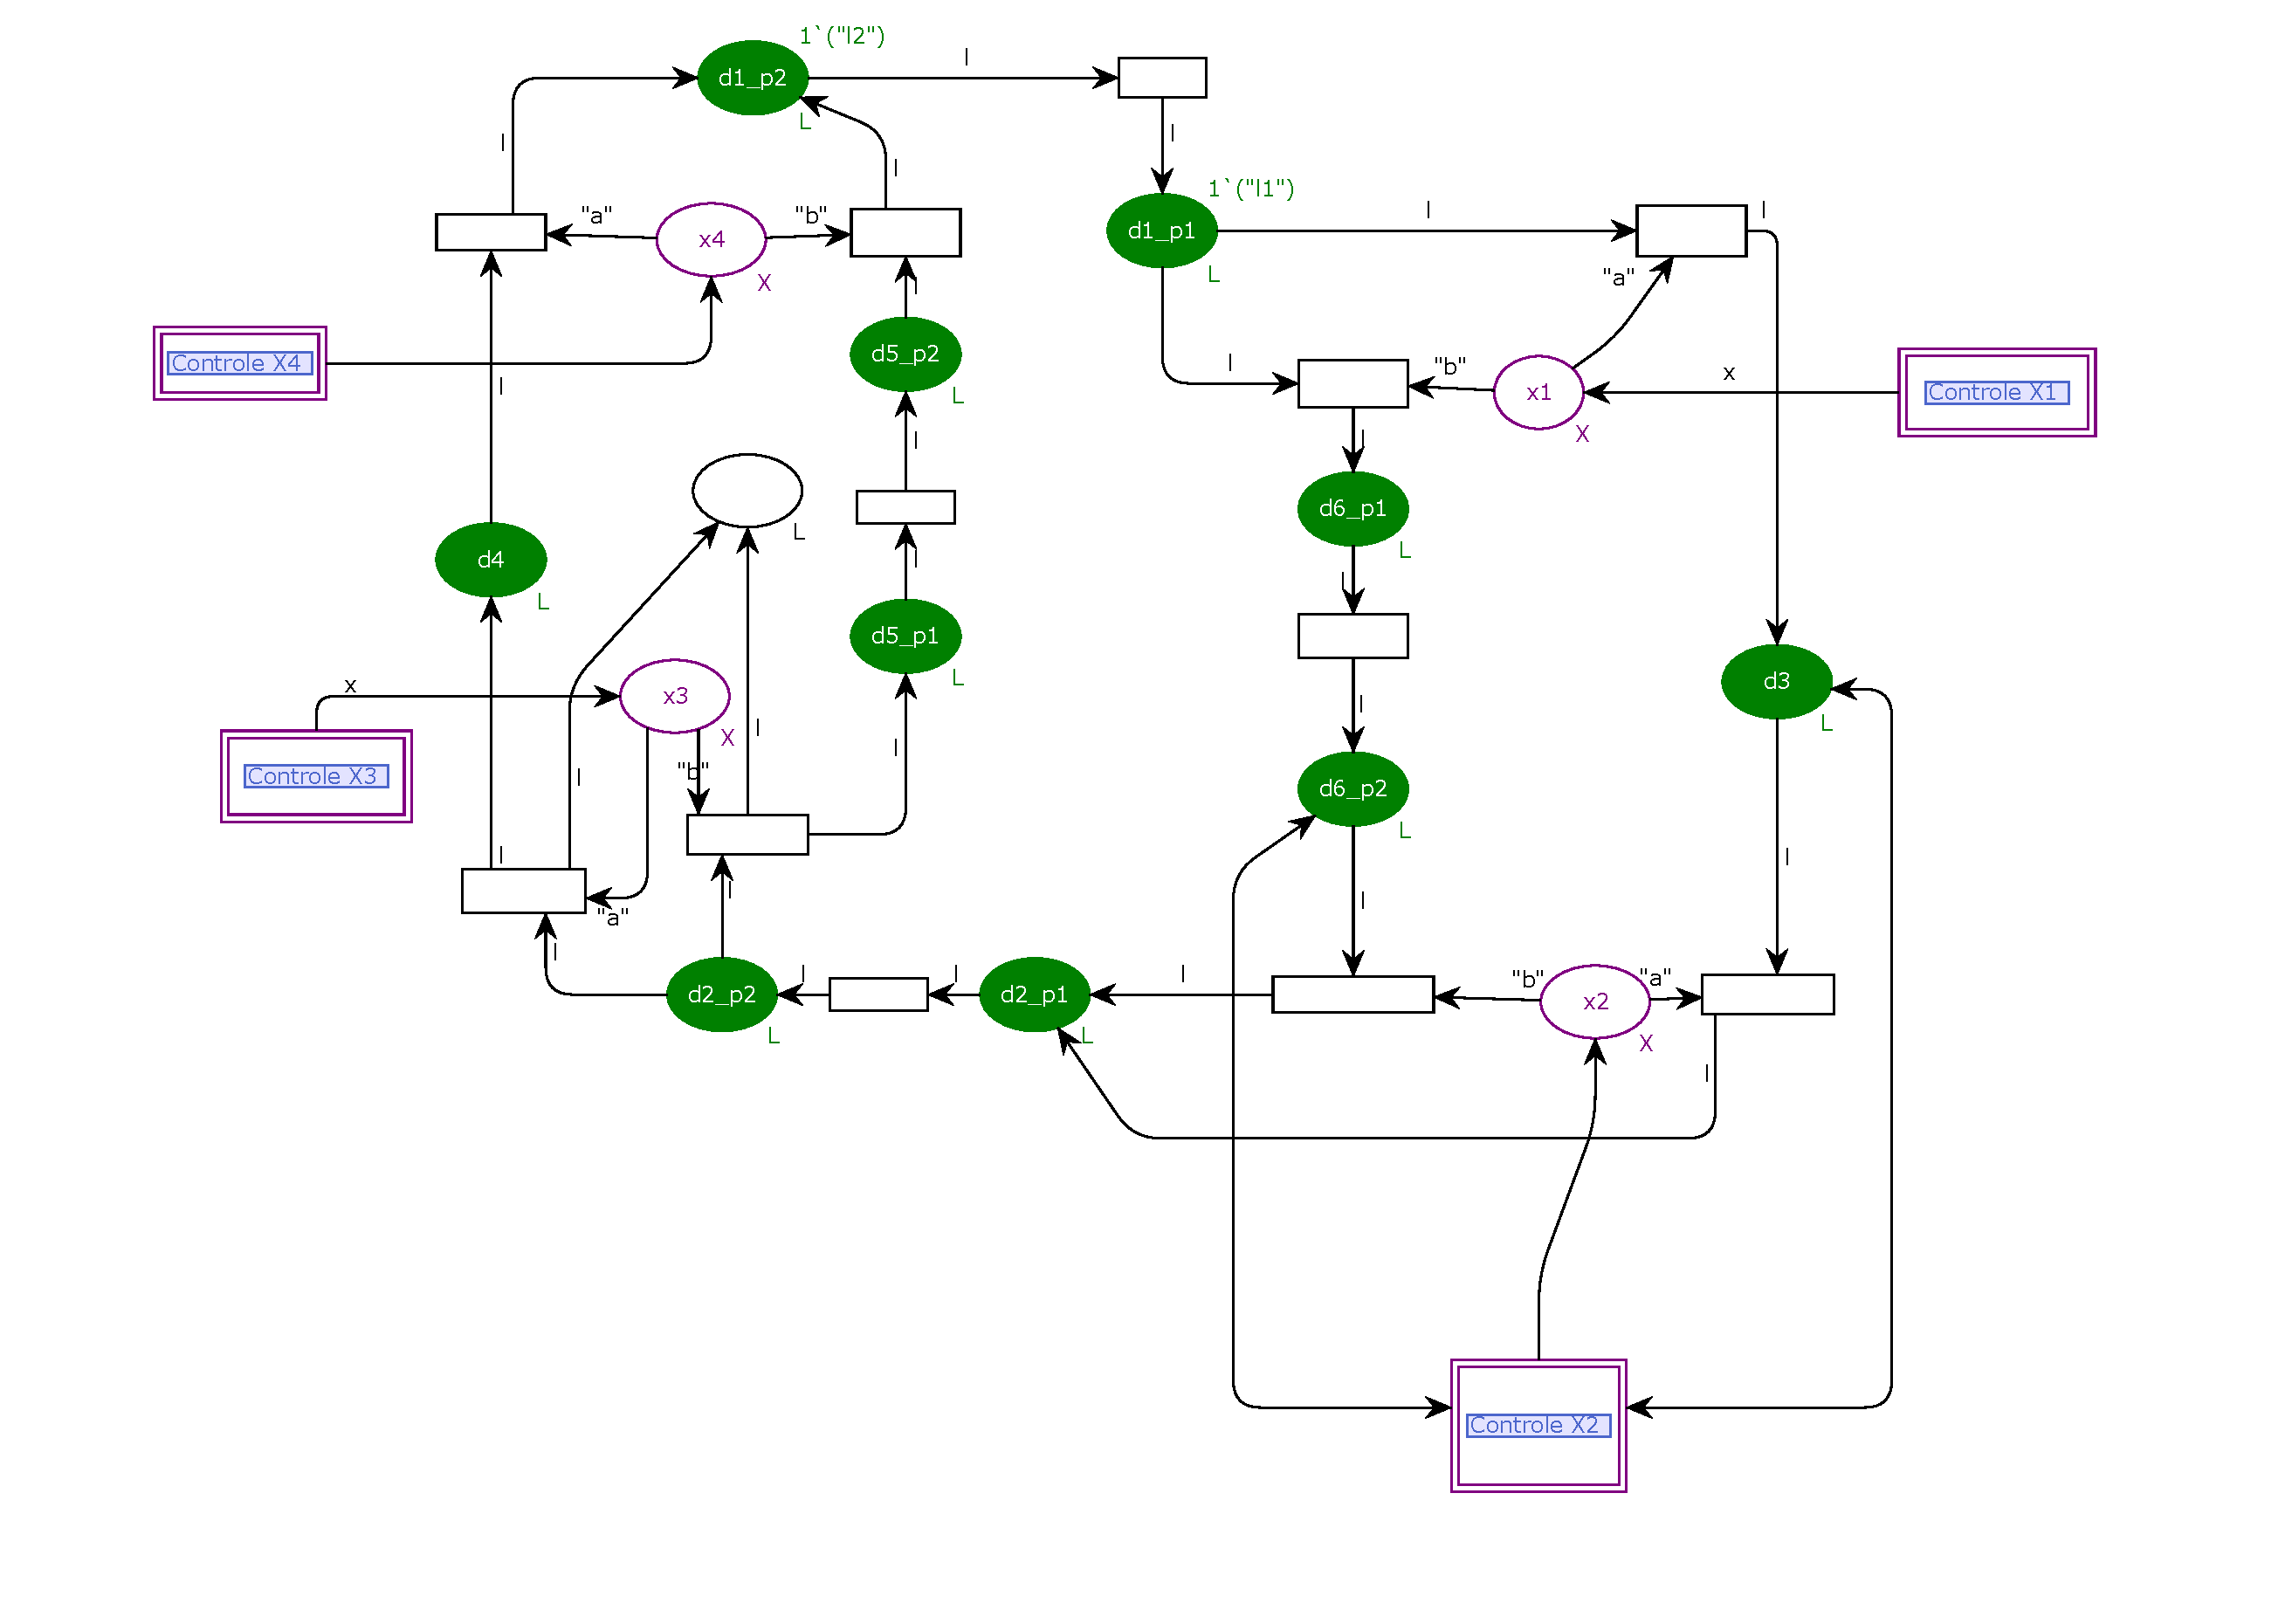
\includegraphics[width=1\linewidth]{figures//Simulation//Modelagem/pista_com_chaves.eps}
    \legend{Fonte: Elaborado pelo autor.}
\end{figure}

Na modelagem dos controladores, é essencial assegurar a comunicação entre os elementos da pista em certos momentos, permitindo que os controladores tomem decisões com base nas posições dos vagões. Um exemplo dessa comunicação é ilustrado na Figura \ref{fig:free_control}. Em algumas transições conectadas às chaves, a informação sobre qual vagão passou pela região é transmitida à medida que as transições são acionadas. Posteriormente, essas informações são fornecidas, direta ou indiretamente, aos controladores.

Por exemplo, note que nas transições ligadas ao lugar $X_2$ possuem lugar de saída definida no conjunto L, de modo que ao passar algum vagão naquela região, a informação de qual vagão passou é processada pelo \textit{Controle} $X_2$. Posteriormente ao se passar os dois vagões diferentes a transição ligada ao lugar \textit{free} $x_3$ é habilitada, transmitindo a informação de que já se passaram aqueles dois tipos de vagões naquela região, para a tomada de decisão do \textit{Controle} $X_3$.

\begin{figure}[ht]
    \centering
    \caption{Máscara dos Componentes de controle das chaves e comunicadores na RPC}
    \label{fig:free_control}
    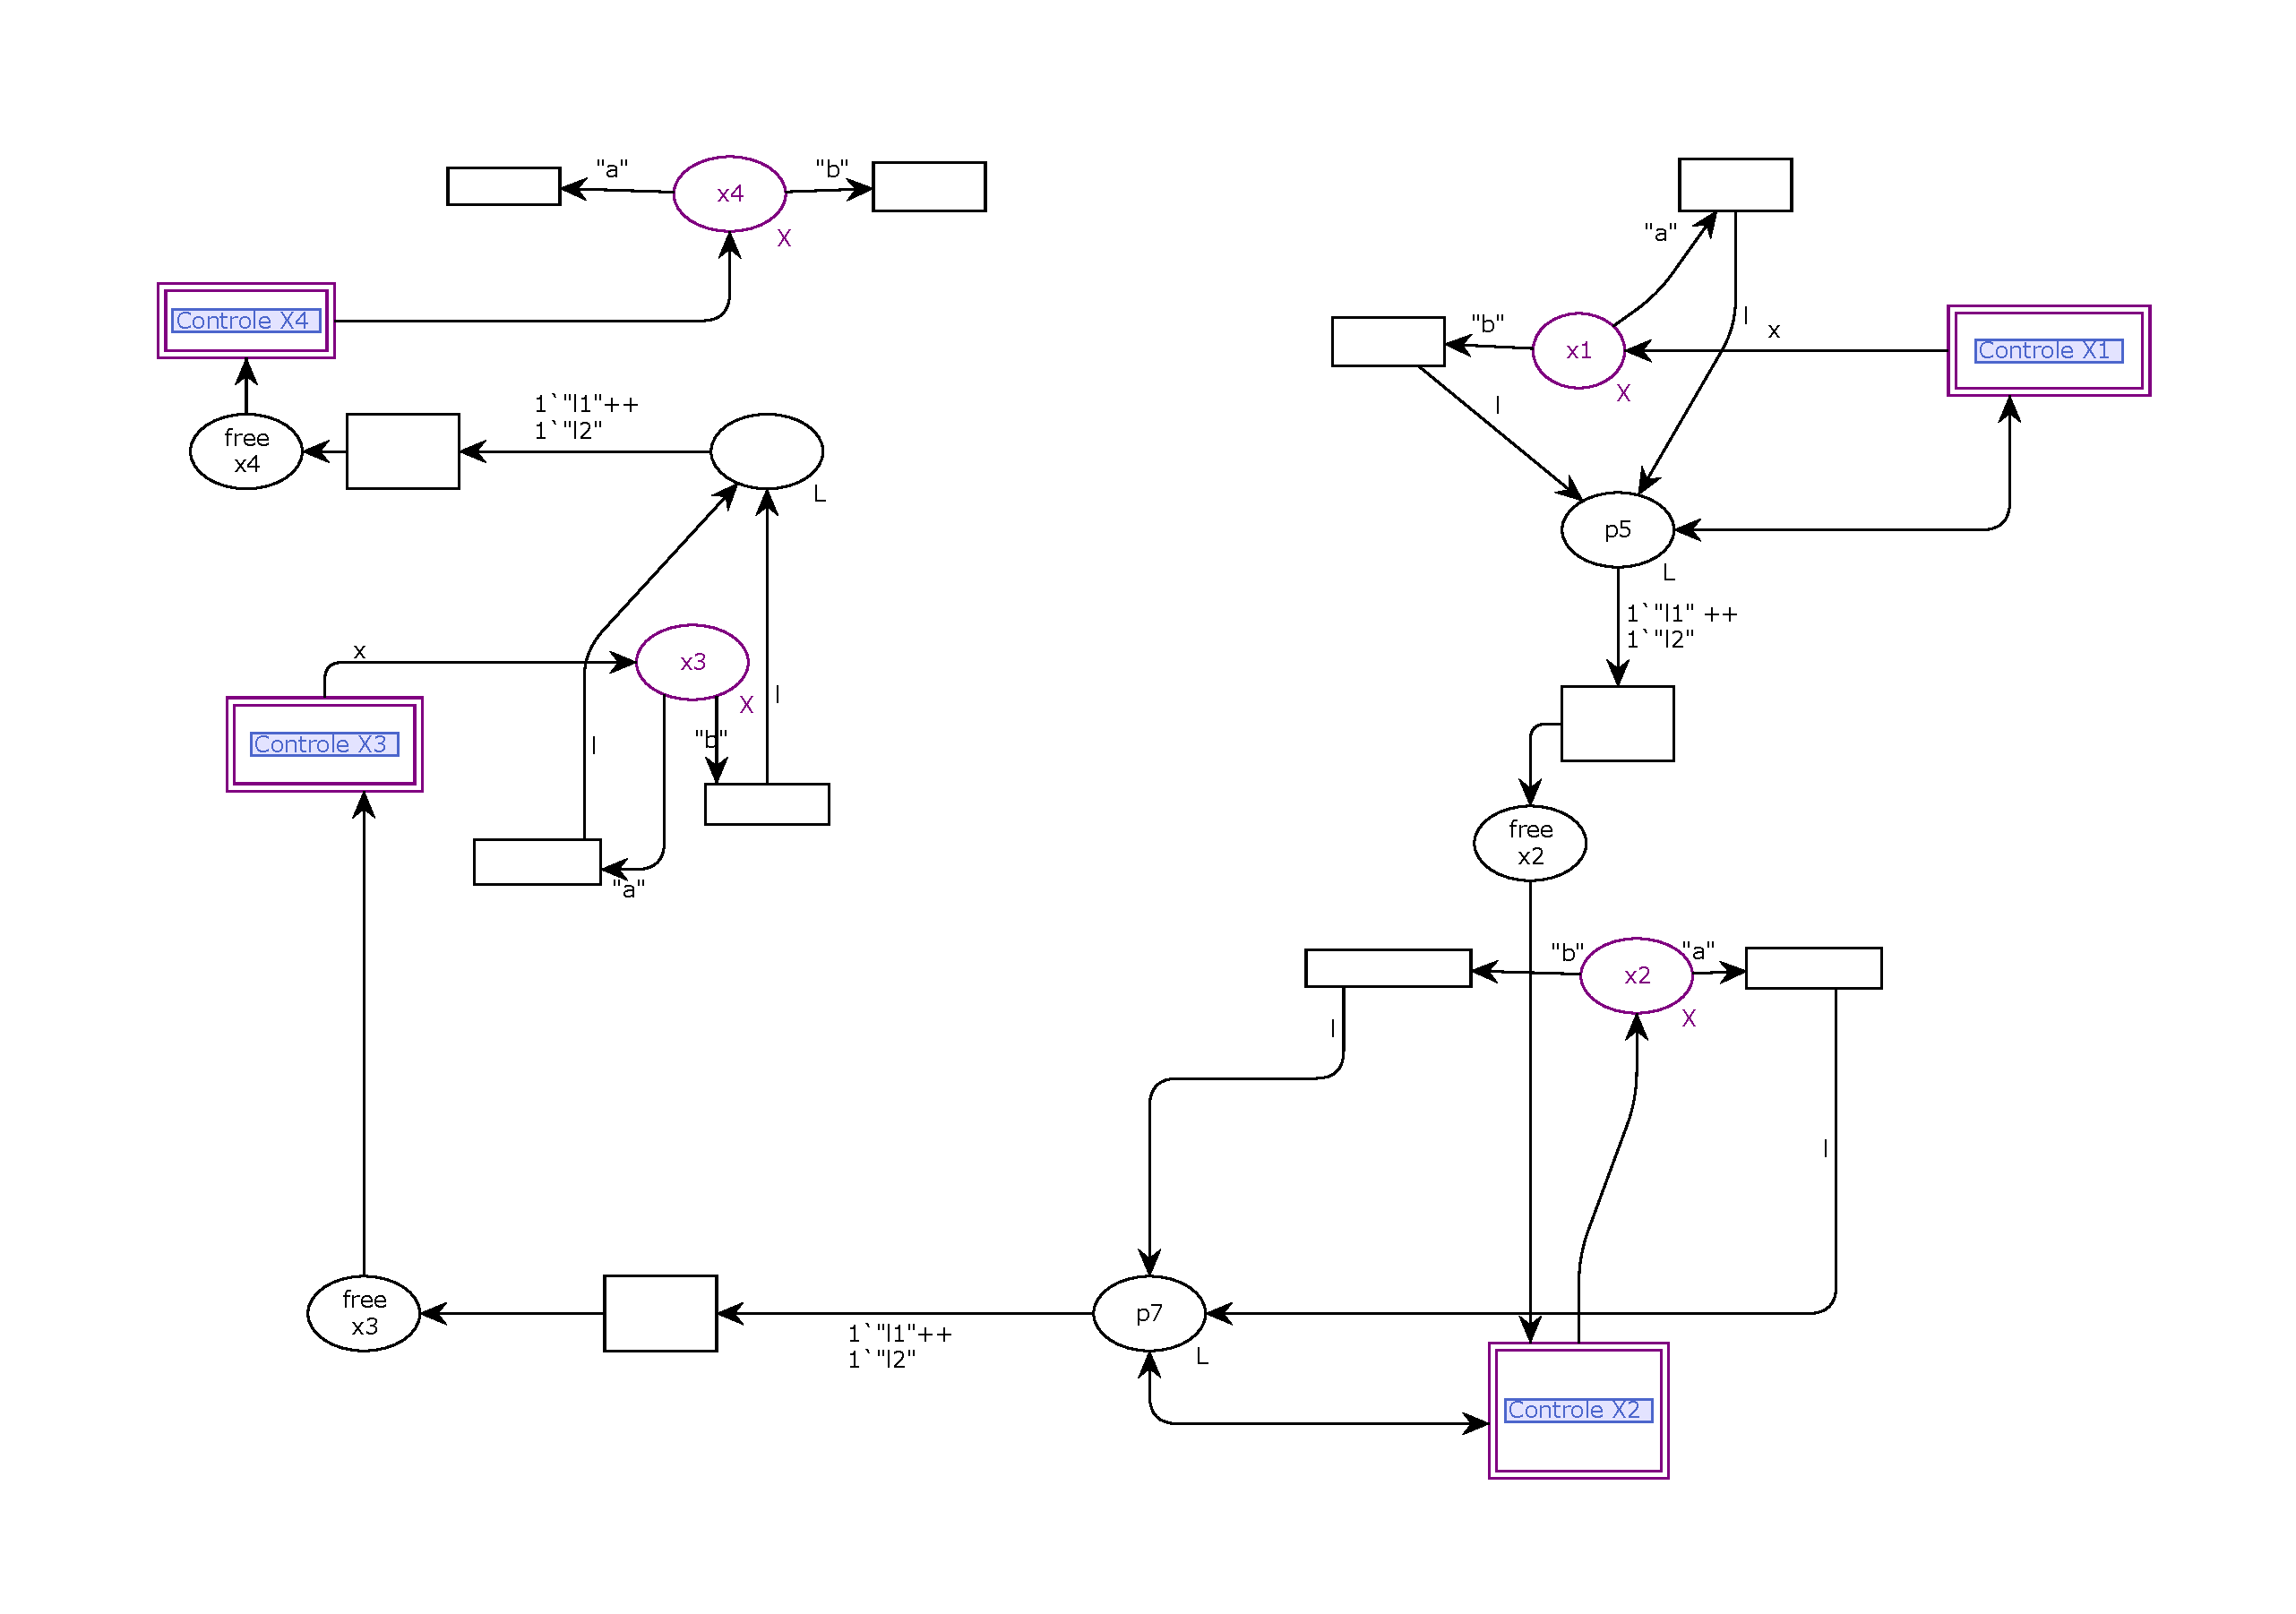
\includegraphics[width=1\linewidth]{figures//Simulation//Modelagem/free_control.eps}
    \legend{Fonte: Elaborado pelo autor.}
\end{figure}


Em um nível hierárquico abaixo do nível da pista, como demonstrado na figura \ref{fig:hierarquia_RPC} estão os \textit{Controladores} $x_1$ a $x_4$, que serão detalhados a seguir. 

O \textit{Controlador} $X_1$ referente a transição \textit{Controle} $X_1$ com borda vermelha na figura \ref{fig:free_control}, é demonstrado na figura \ref{fig:controle_x1}. Note que a rede de Controle de $X_1$, possui alguns lugares com subscrição denominadas de \textit{IN}, \textit{OUT} ou \textit{IN/OUT}, que são diretamente relacionadas aos lugares externos a rede, estabelecendo uma comunicação com lugares pertencentes ao nível hierárquico superior. Alguns lugares como $x1$ e $p5$ já foram demonstrados na máscara de componentes na figura \ref{fig:free_control}, outros serão demonstrados na subseção \ref{sub:model_ord} referente a modelagem de ordenação dos vagões.

Para o controle do lugar $X_1$ note que a rede possui inicialmente uma ficha no lugar $p_1$, de modo que dependendo do comando de ultrapassar ou não ultrapassar a transição $t_2$ ou $t_1$ será acionada, respectivamente. O acionamento primeiro coloca ficha de posição "a" ou "b" na chave $X_1$ e posteriormente a posição "b" pela transição $t_3$ pós a passagem do primeiro vagão sinalizada pelo lugar $p_5$. Após os dois comandos de posição serem utilizados a rede aguarda o comando externo de restabelece o controle para assim, reiniciar a rede para o estado inicial e começar um novo ciclo.

\begin{figure}[ht]
    \centering
    \caption{Rede referente ao controle hierárquico X1 na RPC}
    \label{fig:controle_x1}
    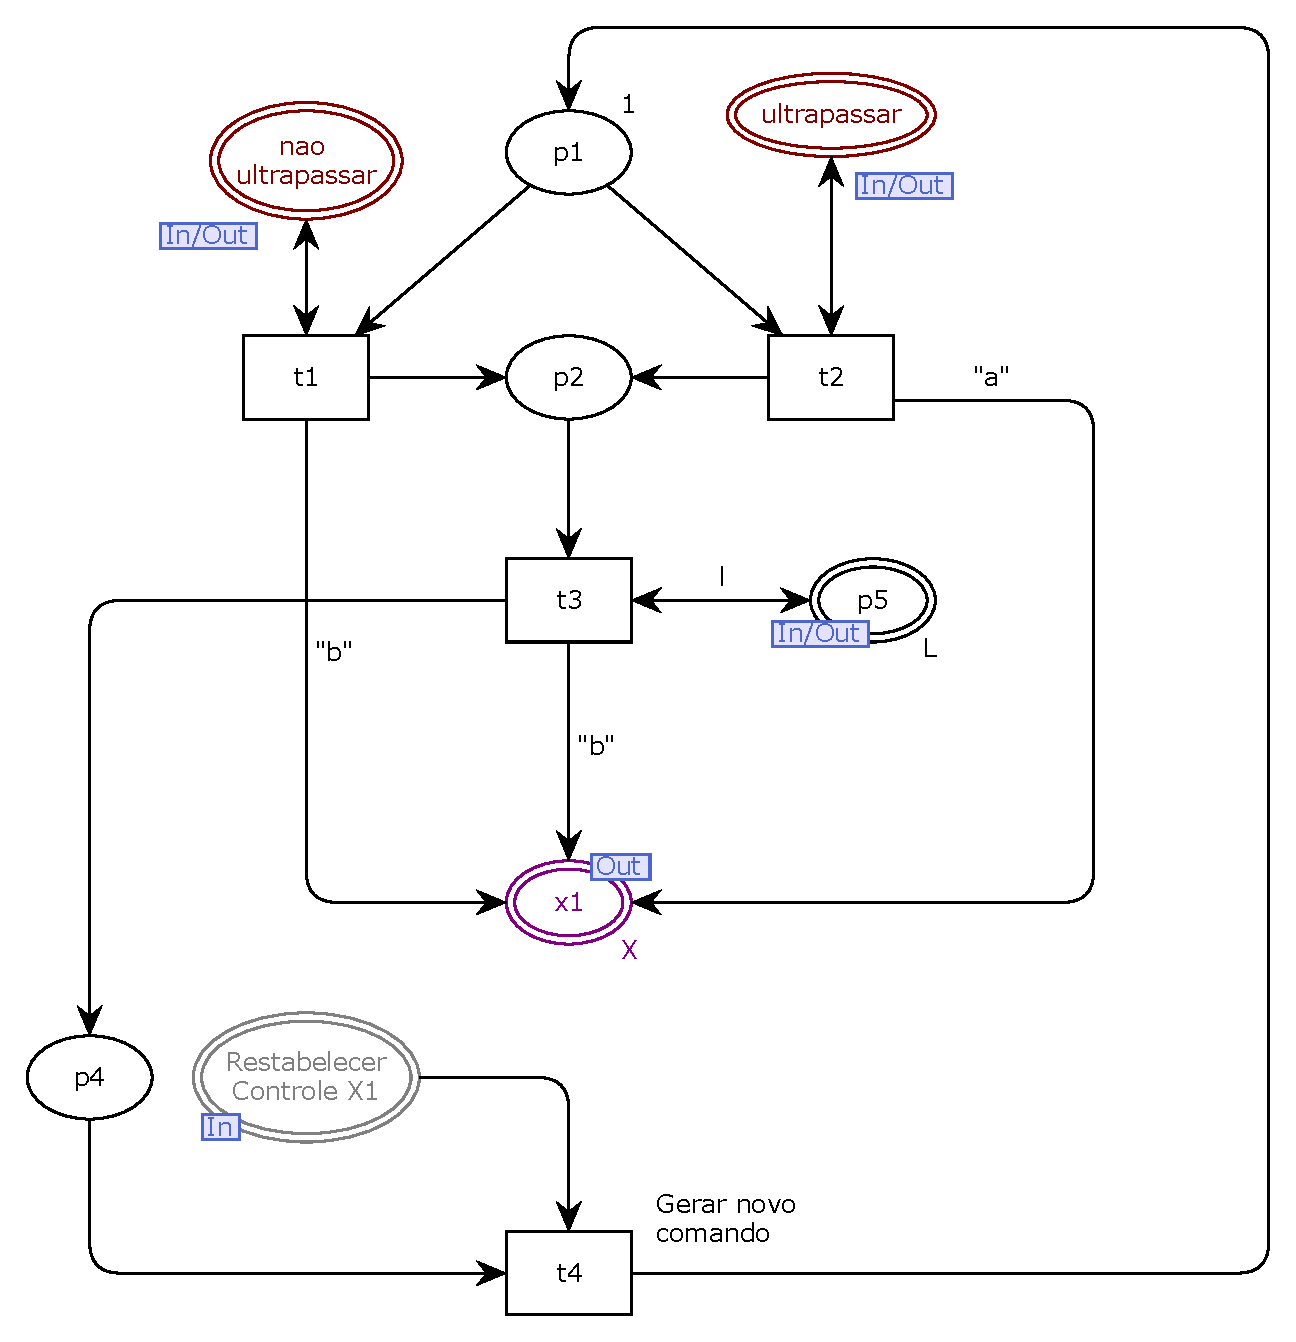
\includegraphics[width=0.5\linewidth]{figures//Simulation//Modelagem/controle_x1.eps}
    \legend{Fonte: Elaborado pelo autor.}
\end{figure}

A RPC referente a transição \textit{Controle} $X_2$ é demonstrado na figura \ref{fig:controle_x2}. Tal controle tem como objetivo primeiramente receber o vagão da pista $d_6$, ou seja do menor caminho e posteriormente, analisar caso tenha tido o comando de ultrapassagem o próximo vagão é esperado na pista $d_3$, caso contrário virá novamente pela pista $d_6$. Para alcançar tal objetivo primeiramente a estrutura da rede recebe uma ficha vinda da pista de \textit{free} $x_2$ ativando a transição $t_9$ que espera o vagão chegar em $d_6$, ao ser identificado na curva é liberada primeiramente a ficha para X2 "b". Posteriormente, dependendo do comando relacionado à ultrapassagem é acionado $t_13$ ou $t_12$, com as fichas respectivamente em $p_11$ ou $p_10$, é esperado que chegar uma ficha no lugar $p_7$ indicando que já pode dar o segundo comando para a chave, por fim é dado o comando de posição "a" ou "b" para a chave caso $t_8$ seja acionado ou $t_7$, respectivamente. Ao fim do ciclo a rede espera uma ficha para restabelecer o \textit{Controle} $X_2$.

\begin{figure}[ht]
    \centering
    \caption{Rede referente ao controle hierárquico X2 na RPC}
    \label{fig:controle_x2}
    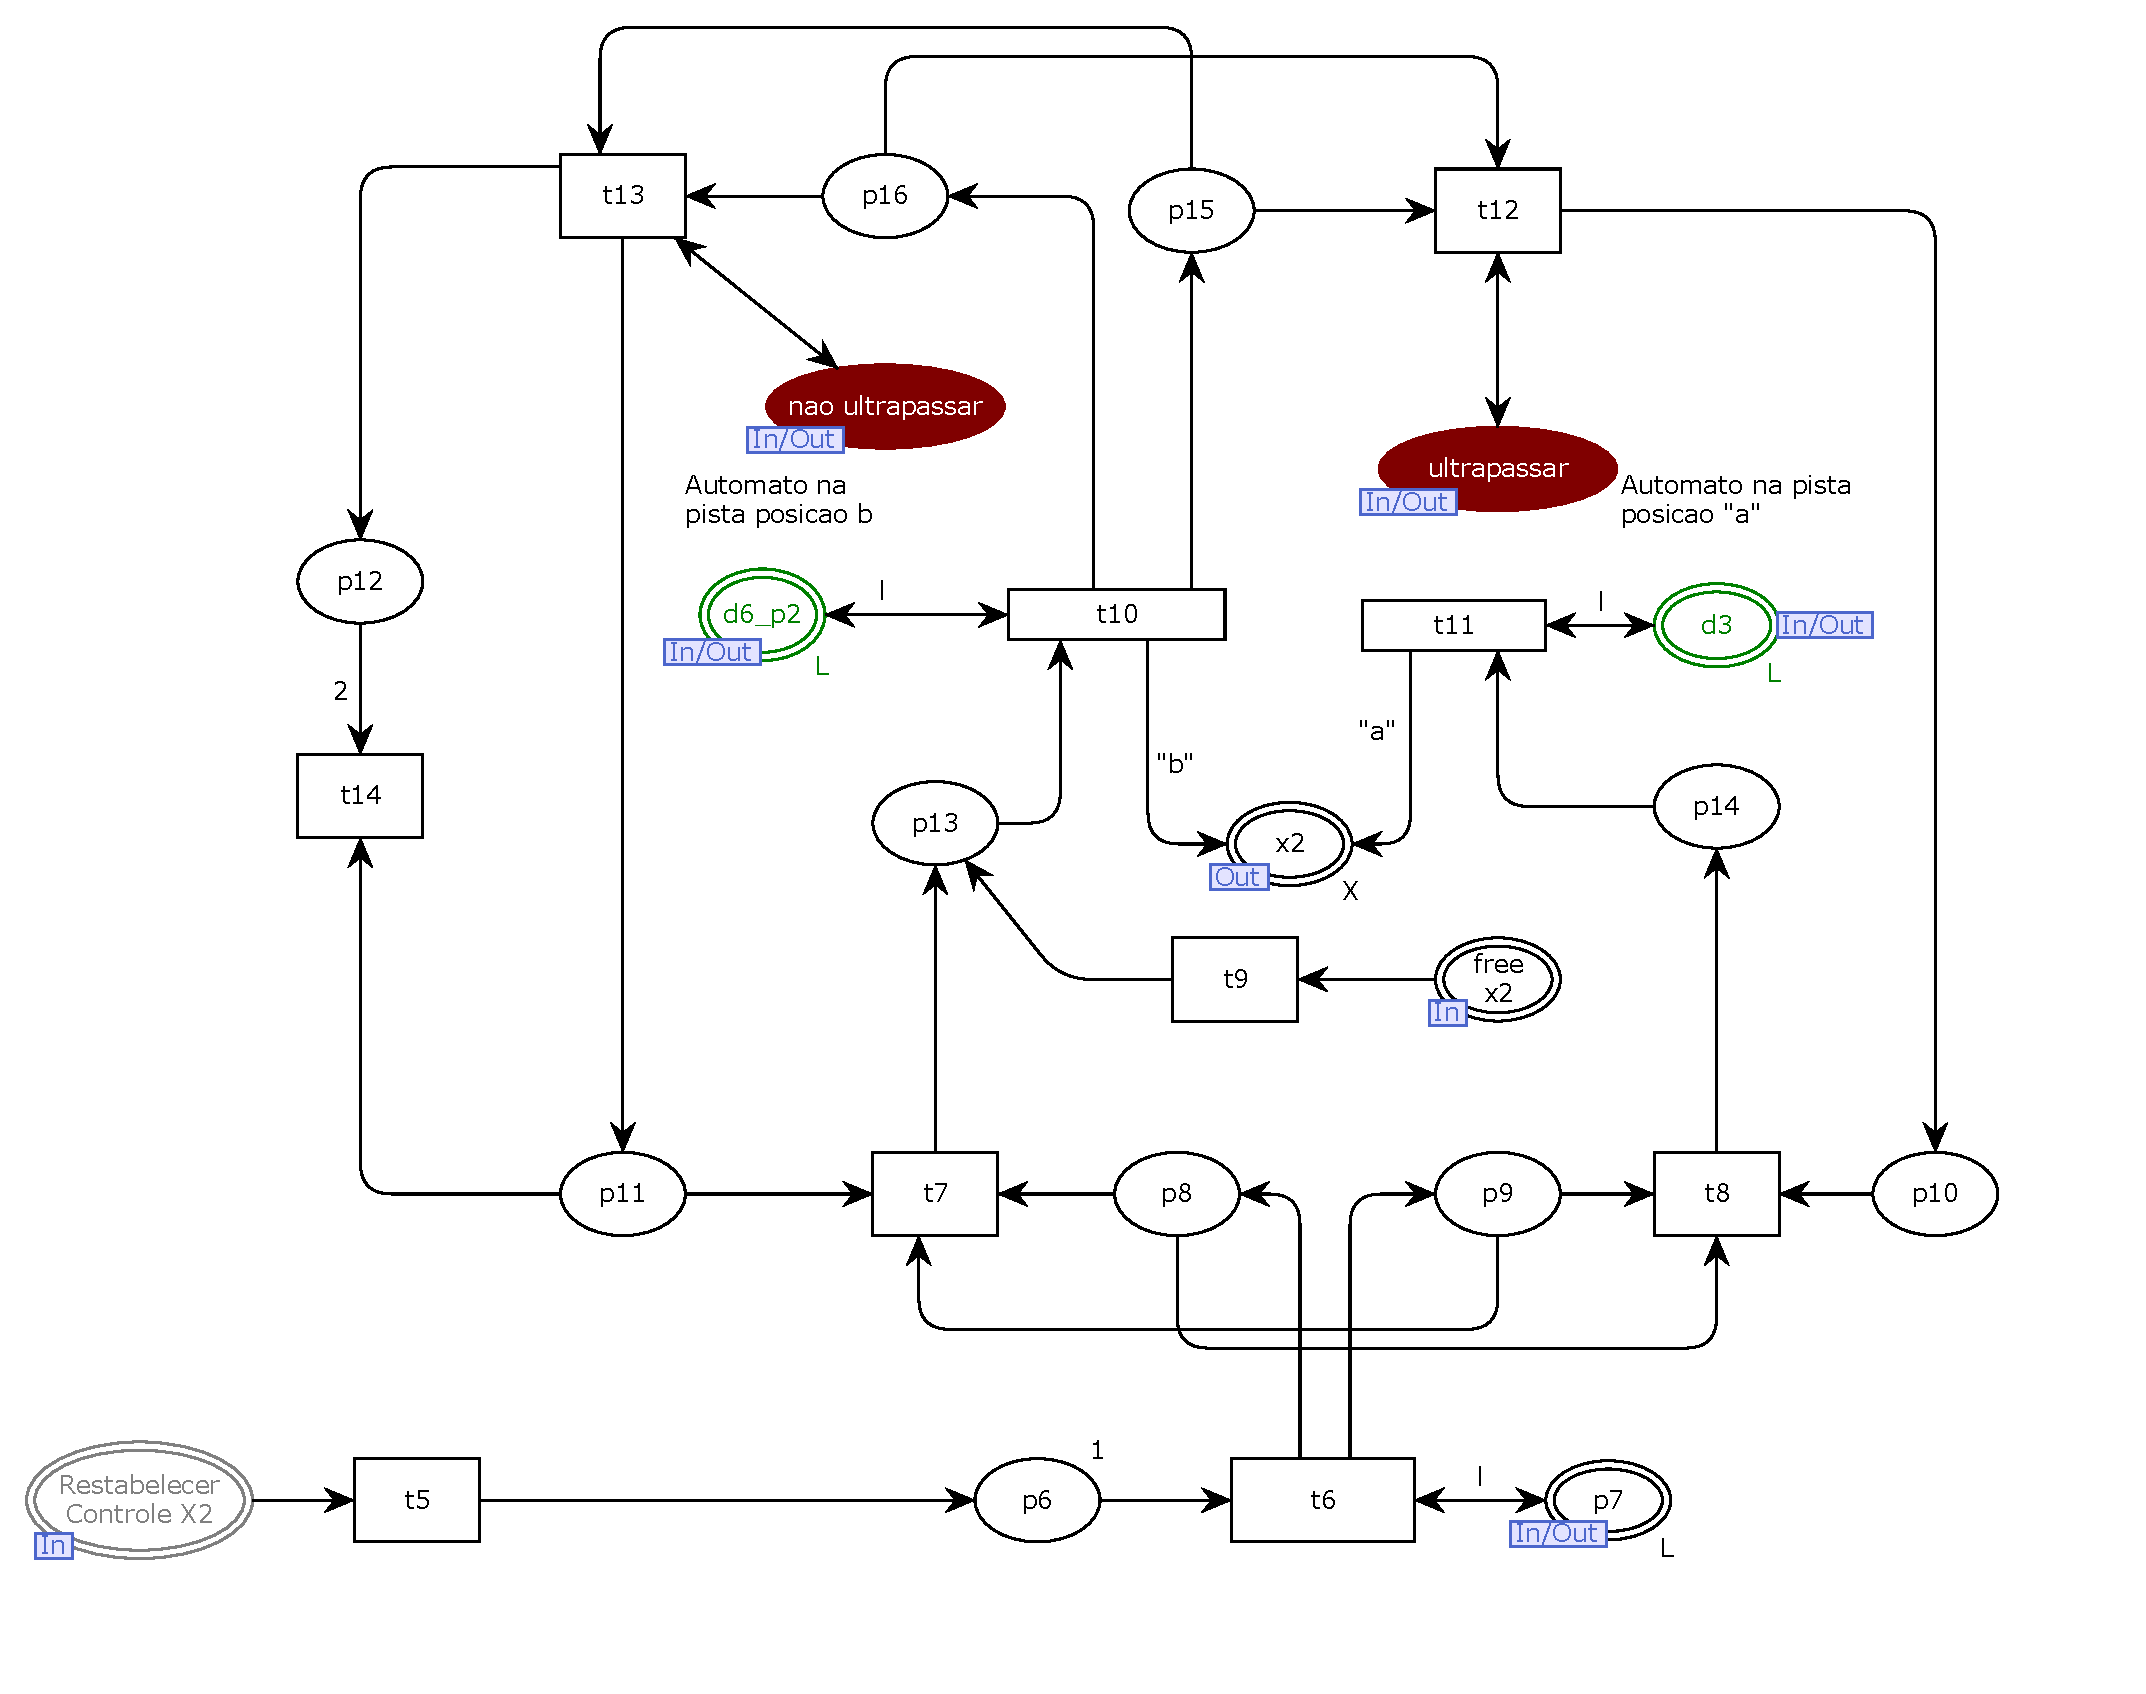
\includegraphics[width=0.9\linewidth]{figures//Simulation//Modelagem/controle_x2.eps}
    \legend{Fonte: Elaborado pelo autor.}
\end{figure}

A RPC referente ao controlador $X_3$ e $X_4$, possuem estruturas e comportamentos idênticos como demonstrados na figura \ref{fig:controle_x3} e \ref{fig:controle_x4}. Como no escopo da simulação o local de ultrapassagem foi fixado no \textit{Controle} $X_1$, o objetivo do \textit{Controle} $X_3$ e \textit{Controle} $X_4$ é apenas garantir que uma vez liberado o controle para o controlador através do lugar \textit{free} $x_3$ ou $x_4$ seja colocada a ficha de posição \textit{"b"}, ou seja o menor caminho para o vagão que vinher.

\begin{figure}[ht]
    \centering
    \caption{Rede referente ao controle hierárquico X3 na RPC}
    \label{fig:controle_x3}
    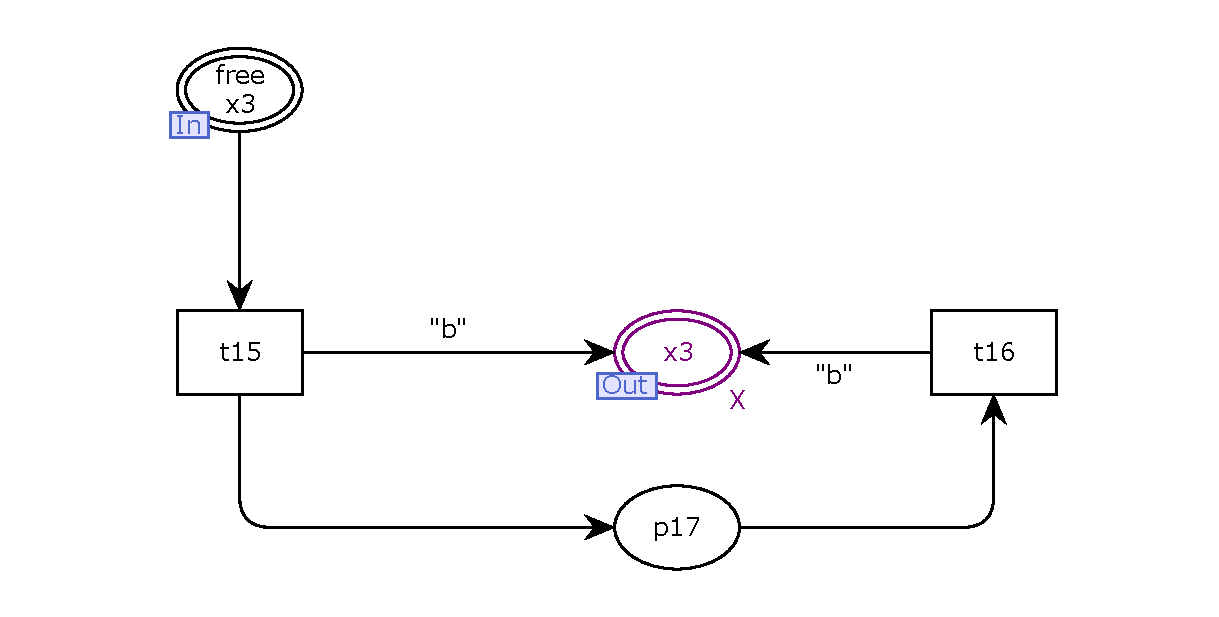
\includegraphics[width=0.6\linewidth]{figures//Simulation//Modelagem/controle_x3.eps}
    \legend{Fonte: Elaborado pelo autor.}
\end{figure}

\begin{figure}[ht]
    \centering
    \caption{Rede referente ao controle hierárquico X4 na RPC}
    \label{fig:controle_x4}
    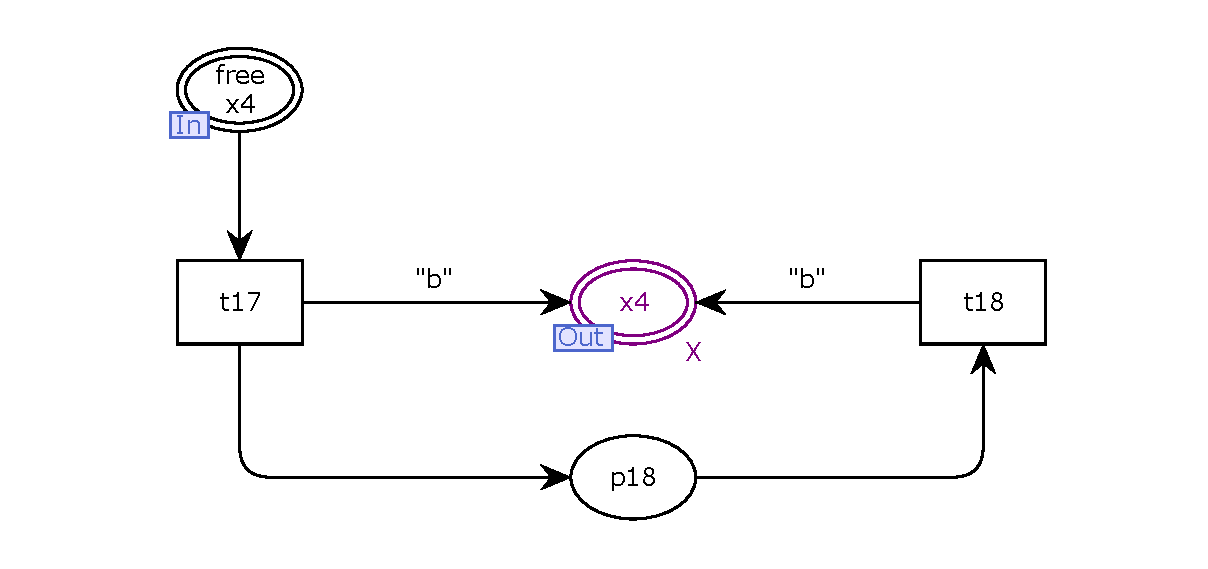
\includegraphics[width=0.6\linewidth]{figures//Simulation//Modelagem/controle_x4.eps}
    \legend{Fonte: Elaborado pelo autor.}
\end{figure}

\clearpage 
\subsection{Modelagem Ordenação dos vagões}
\label{sub:model_ord}
Na hierarquia trabalhada referente a figura \ref{fig:hierarquia_RPC}, que do modelo hierárquico referente a RPC, será demonstrado agora as redes relacionadas aos comando de coordenação dos vagões. Na camada de cima da hierarquia da pista as transições e lugares de ordem e inversão de ordem possuem comunicação principal com os controladores, como demonstrado na máscara do primeiro nível hierárquico na figura \ref{fig:pista_ordem}. Note que as informações de ultrapassagem e não ultrapassagem tem comunicação contro os \textit{Controladores} $X1$ e $X2$ e quem gerencia o primeiro($1_{st}$) e segundo($2_{nd}$) lugar são os dois componentes de \textit{Ordem} e\textit{ Inversão de Ordem}.

\begin{figure}[ht]
    \centering
    \caption{Máscara de componentes relacionados a ordem na RPC}
    \label{fig:pista_ordem}
    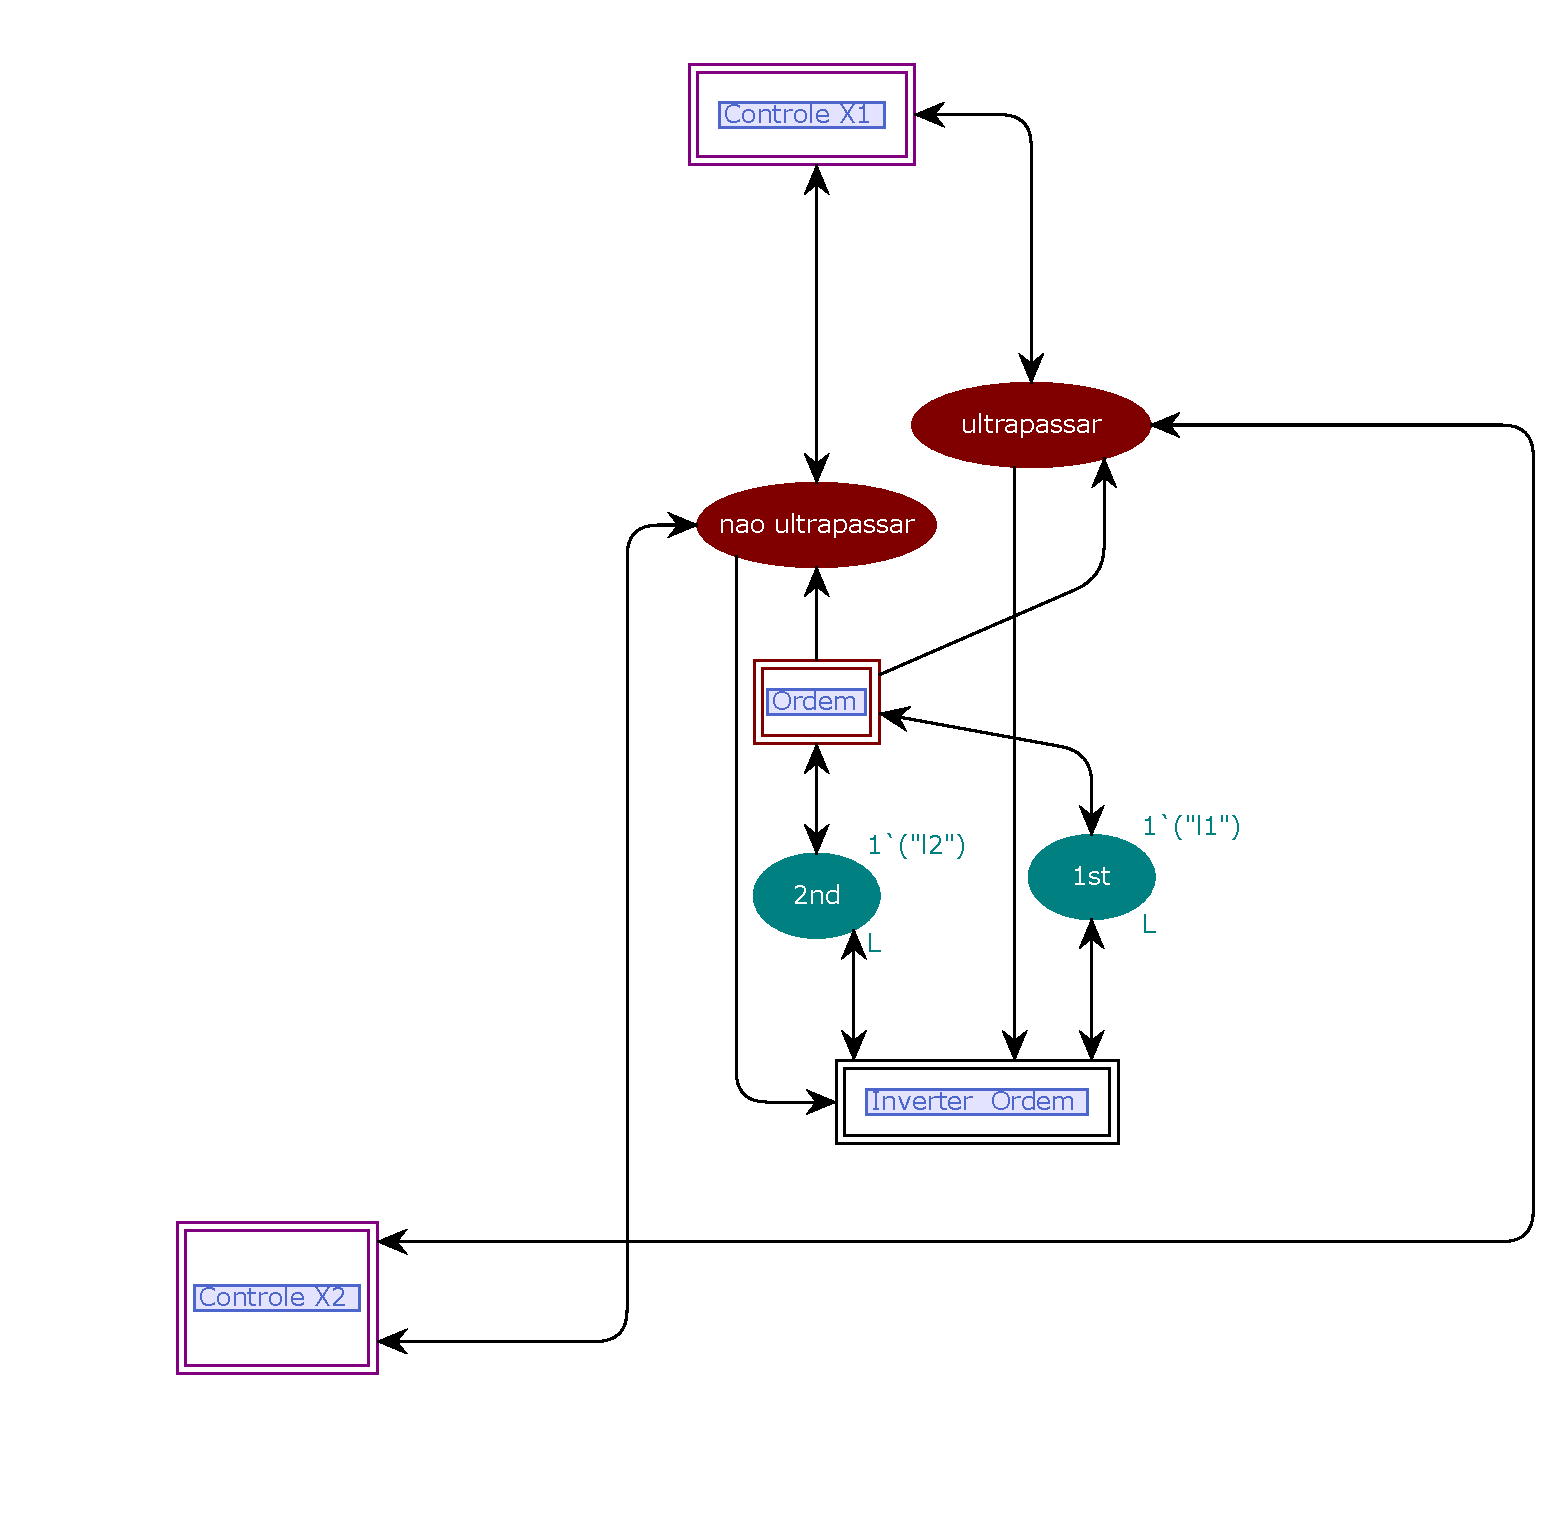
\includegraphics[width=0.8\linewidth]{figures//Simulation//Modelagem/pista_ordem.eps}
    \legend{Fonte: Elaborado pelo autor.}
\end{figure}

A transição hierárquica do componente de \textit{Ordem} é definida através da RPC demonstrada na figura \ref{fig:ordem}, para melhor compreensão a mesma foi dividade em duas máscaras uma de geração de comando e outra de restabelecimento da rede para geração de um novo comando.

\begin{figure}[ht]
    \centering
    \caption{Rede referente ao componente de Ordem na RPC}
    \label{fig:ordem}
    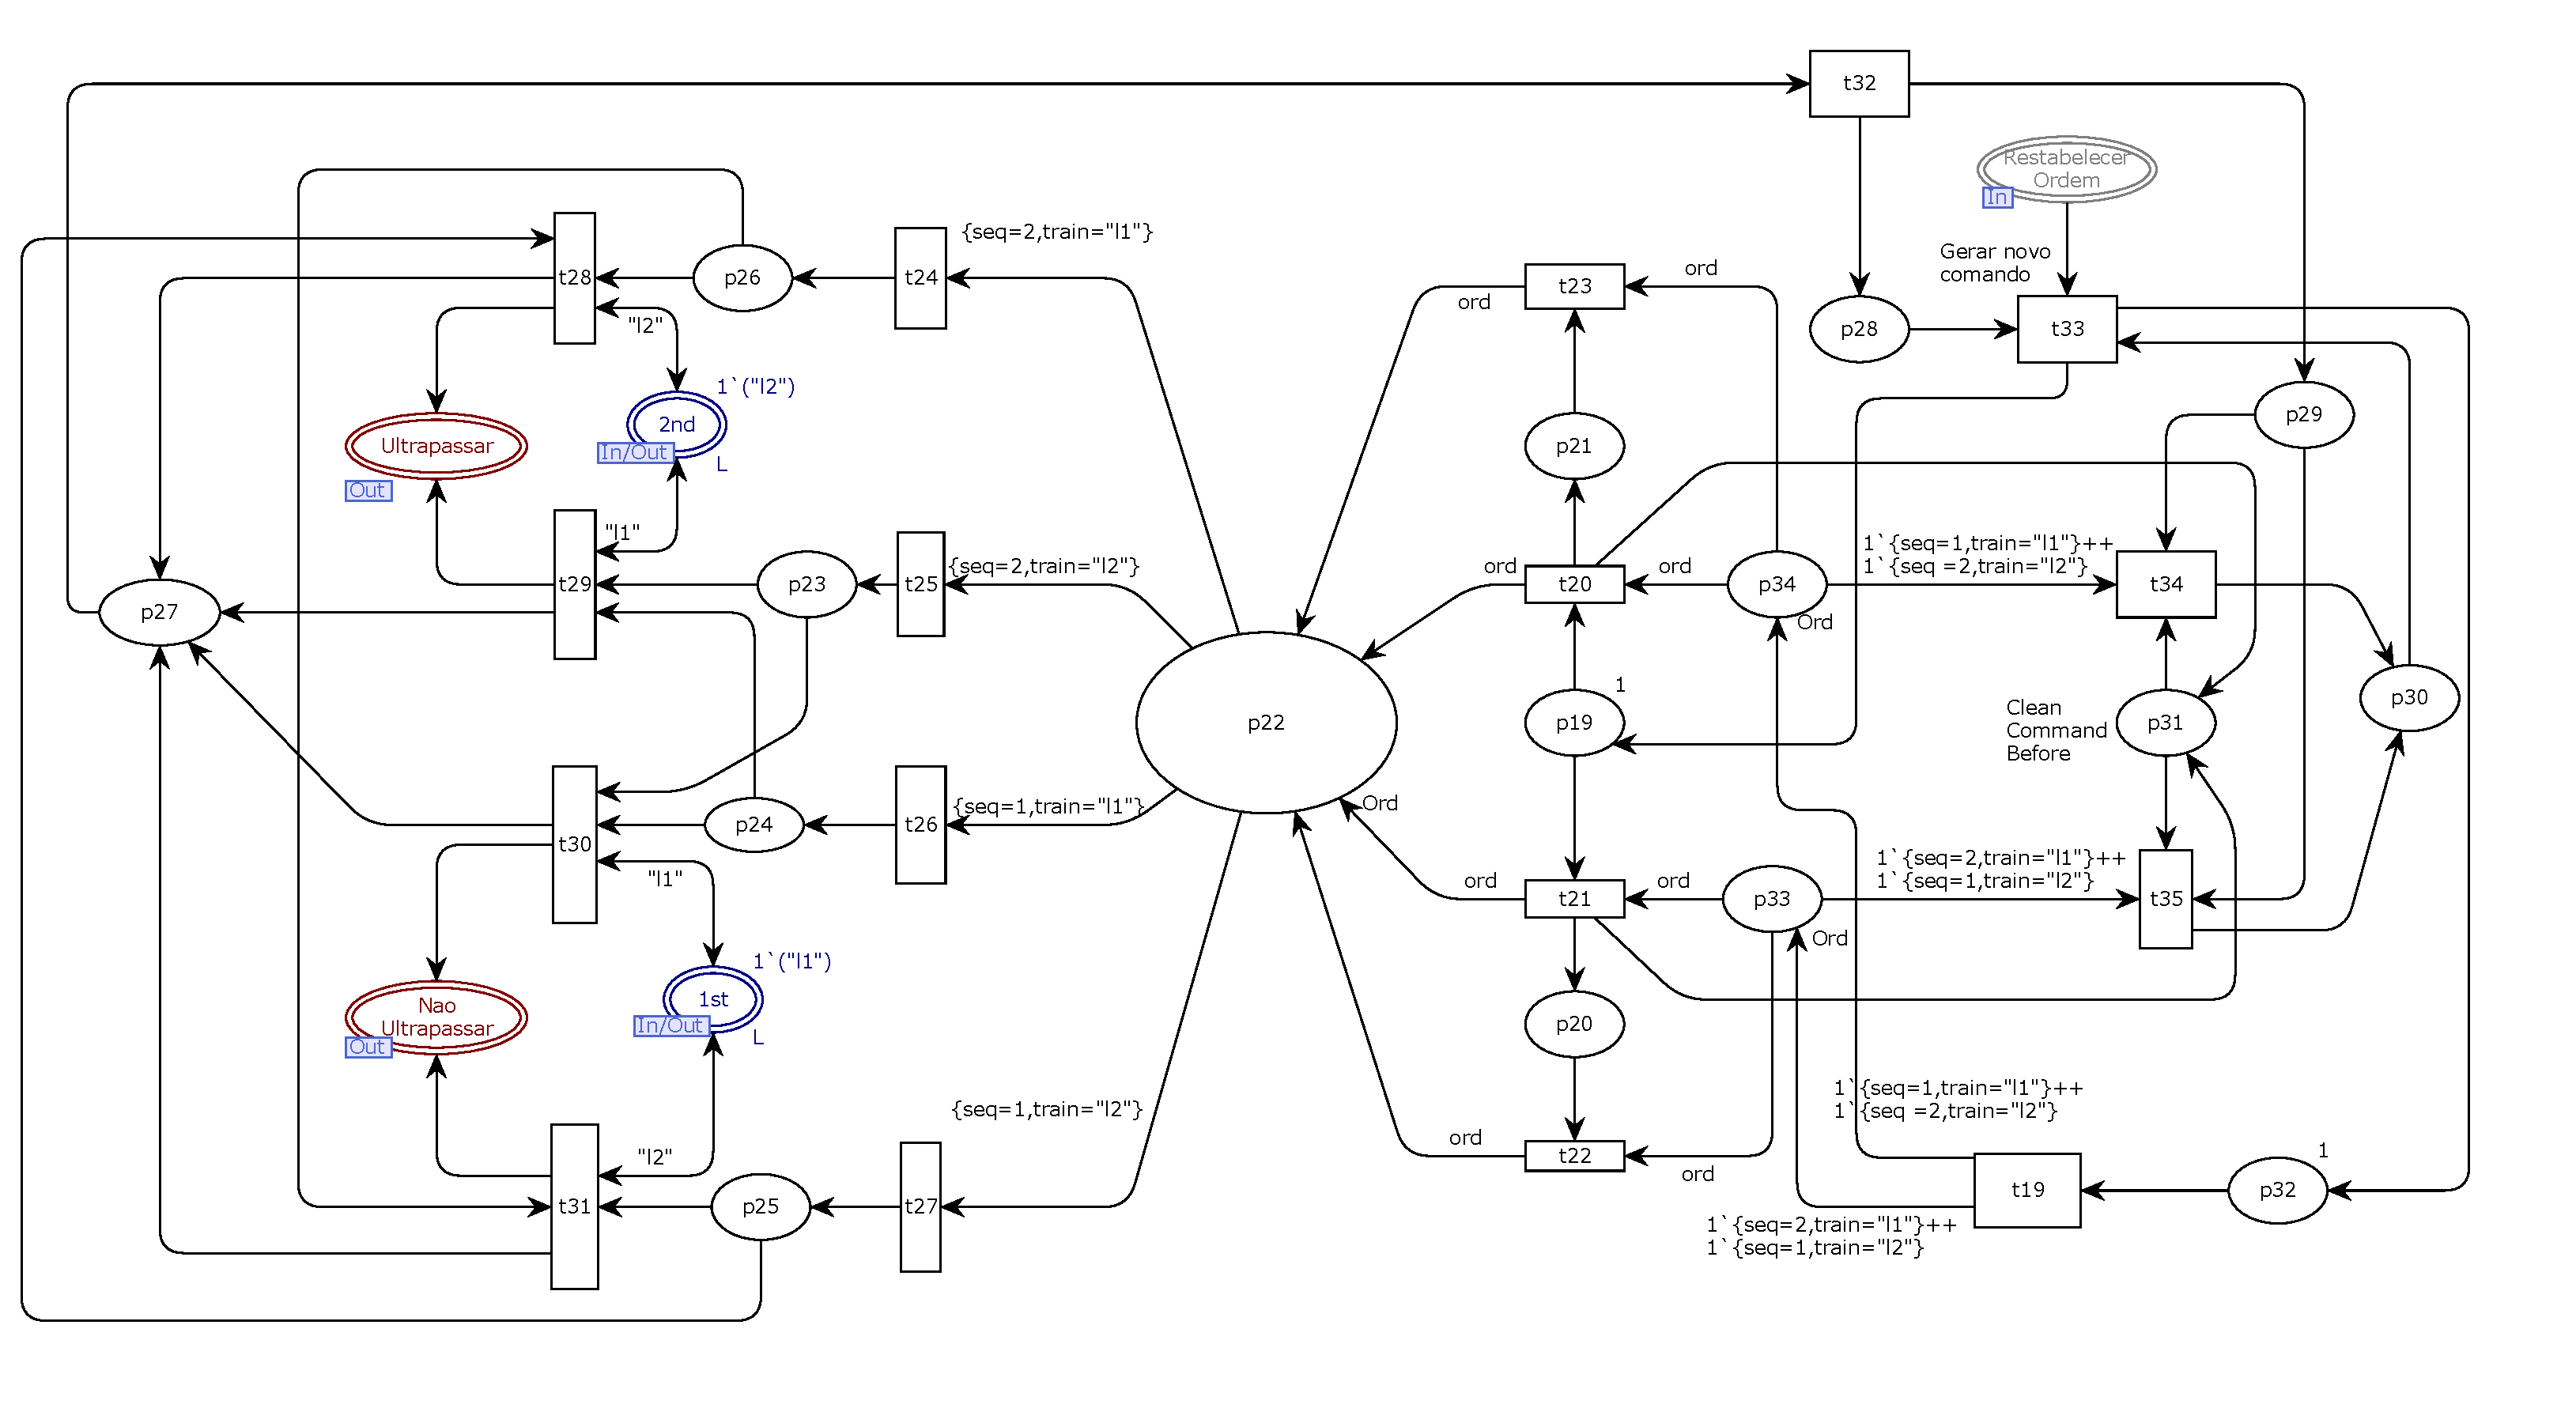
\includegraphics[width=1\linewidth]{figures//Simulation//Modelagem/ordem.eps}
    \legend{Fonte: Elaborado pelo autor.}
\end{figure}

Na geração do comando referente a ultrapassagem ou não ultrapassagem a parte da rede responsável é demonstrada na figura \ref{fig:geracao_ordem}, tal que no início da rede na transição $t_{19}$, são carregados dois comandos o primeiro comando que é recebido pelo lugar $p_{34}$ é o par da do vagão $l_1$ na posição 1 e o vagão $l_2$ na posição 2, através das fichas $1`\{seq=1,train="l1"\} ++ 1`\{seq=2,train="l2"\}$. De modo análogo o segundo comando é recebido pelo lugar $p_{33}$ referente ao vagão $l_2$ na posição 1 e o vagão $l_1$ na posição 2, através das fichas $1`\{seq=2,train="l1"\} ++ 1`\{seq=1,train="l2"\}$
Depois que os lugares $p_{33}$ e $p_{34}$ recebem as fichas as duas transições $t_{20}$ e $t_{21}$ ficam habilitadas ao mesmo tempo, de modo que o acionamento de uma ou outra é feito de forma aleatória. Por fim é feita a verificação de qual vagão está em primeiro e em segundo lugar pelos lugares $1_{st}$ e $2_{nd}$, respectivamente, para a partir disso ser gerado o comando de \textit{Ultrapassar} ou \textit{Não Ultrapassar}.

\begin{figure}[ht]
    \centering
    \caption{Máscara referente a geração de comando do componente de Ordem na RPC}
    \label{fig:geracao_ordem}
    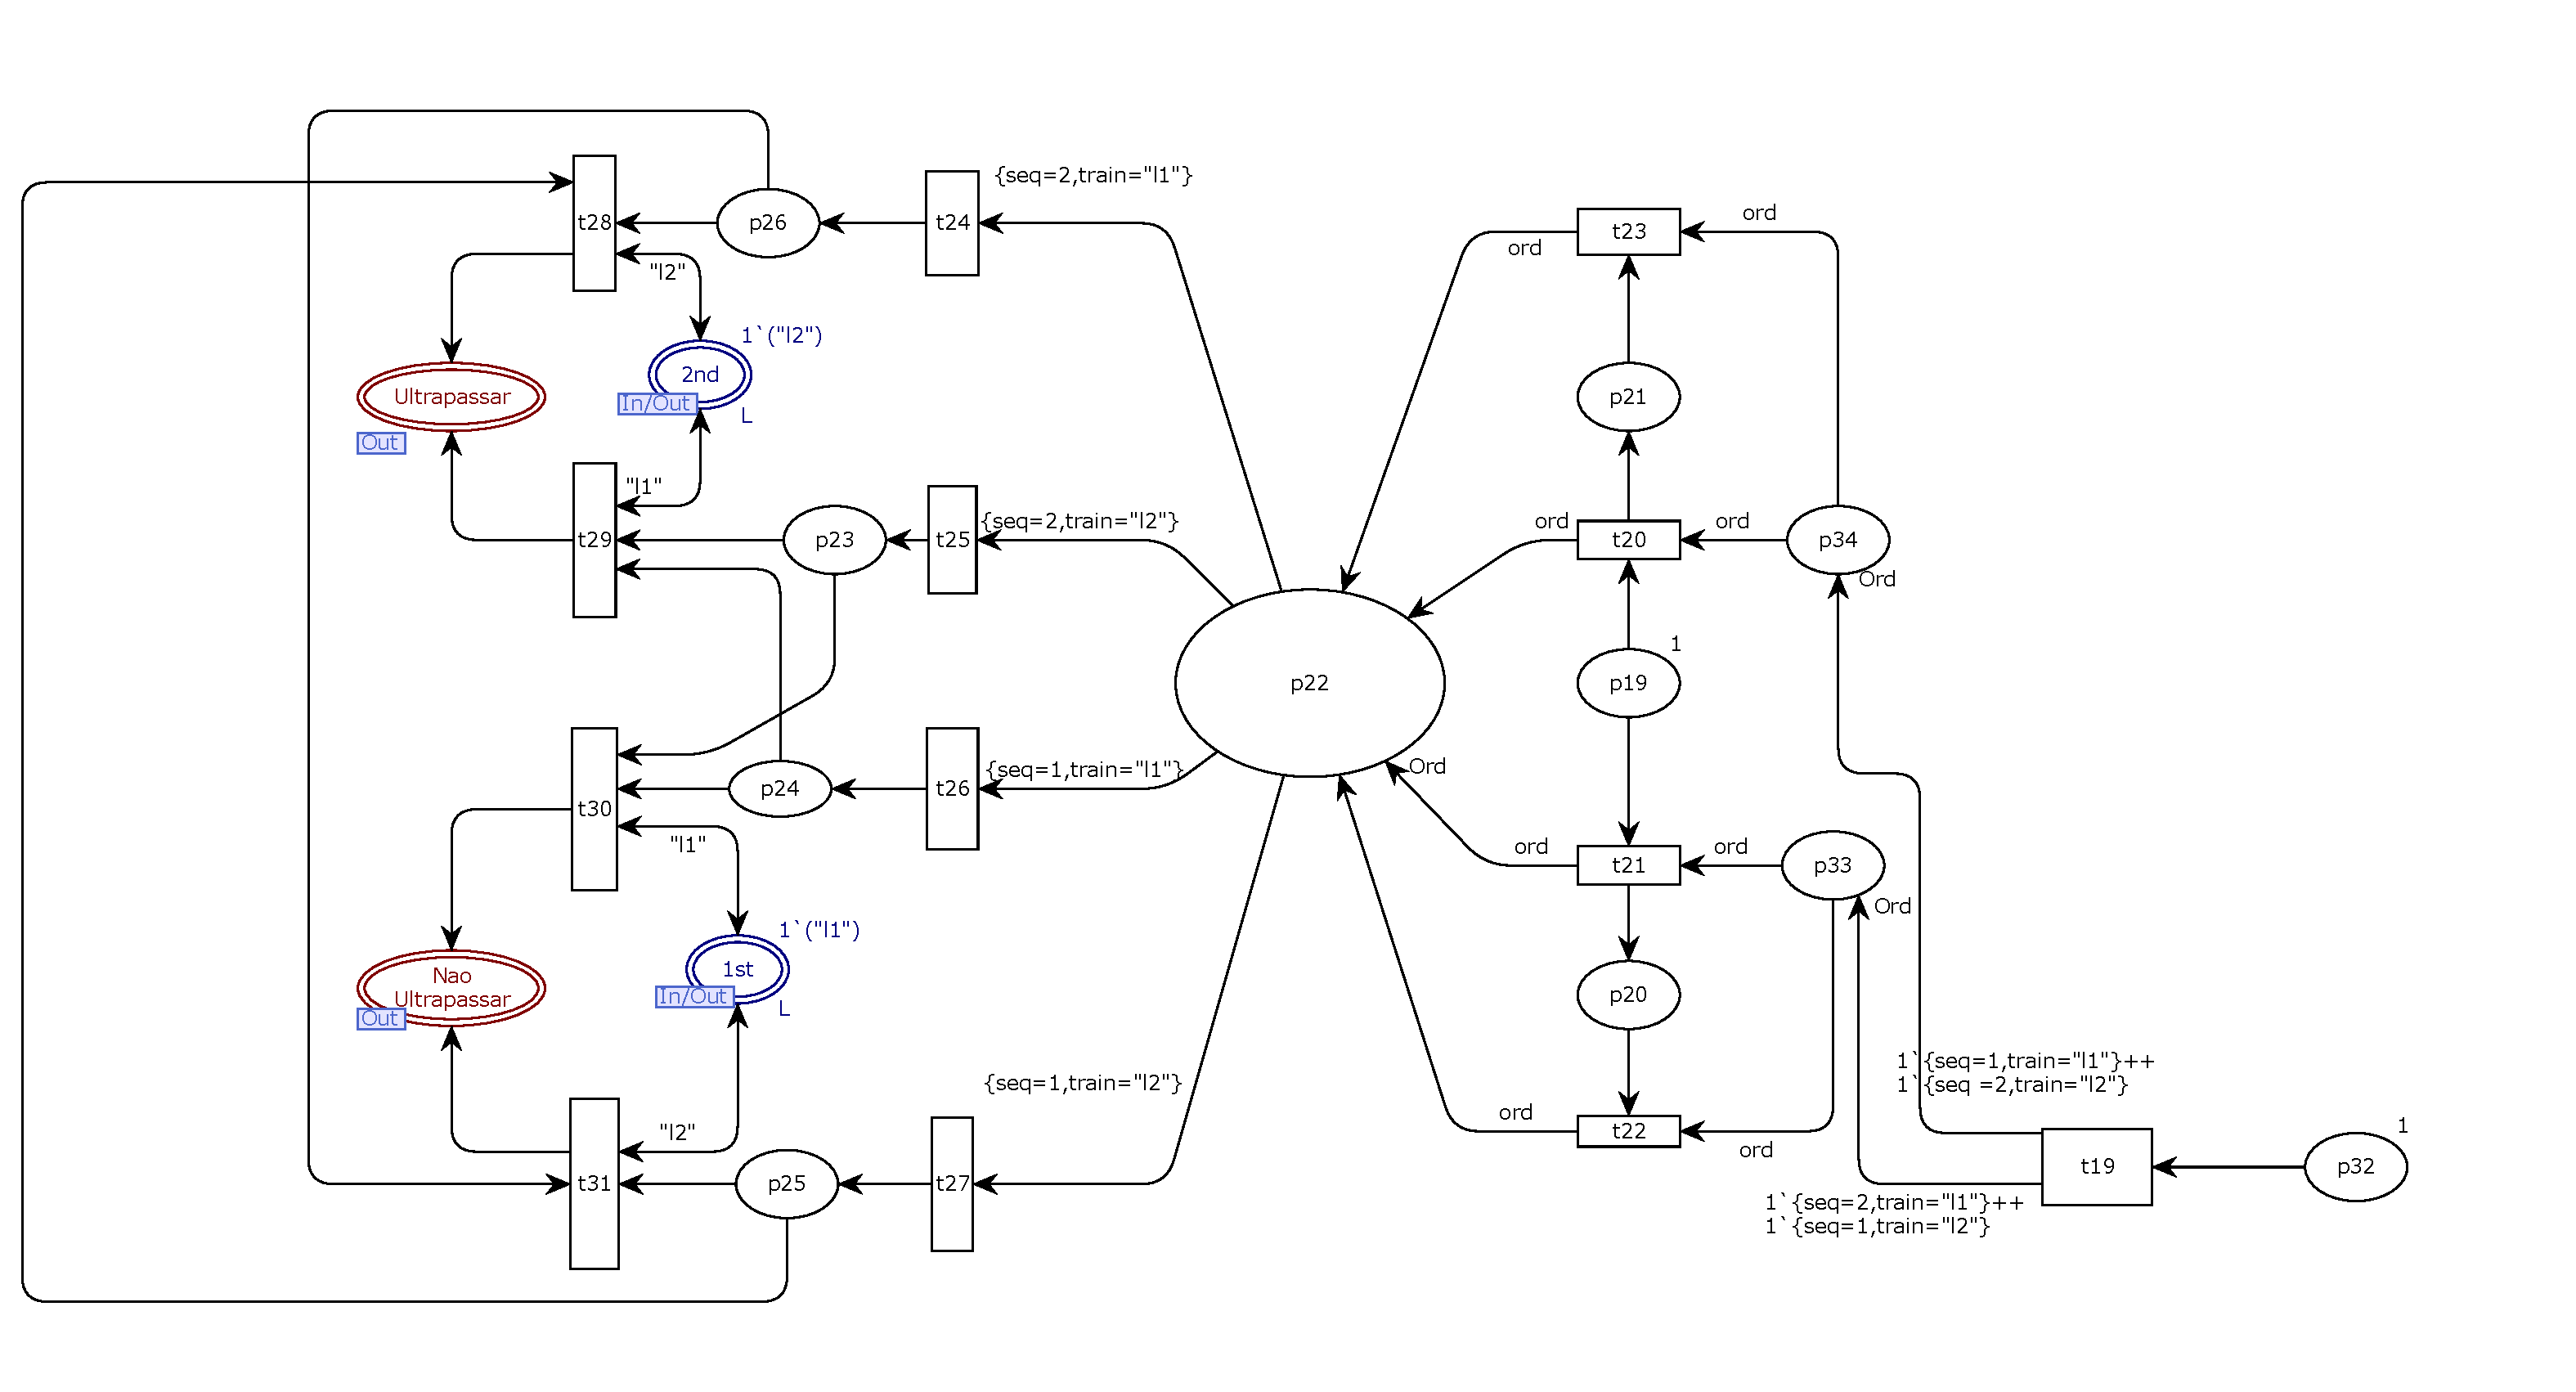
\includegraphics[width=1\linewidth]{figures/Simulation/Modelagem/geracao_ordem.eps}
    \legend{Fonte: Elaborado pelo autor.}
\end{figure}

Após gerado o comando de \textit{Ultrapassar} ou \textit{Não Ultrapassar} é necessário modelar o reestabelecimento da rede para que possa ser gerado novamente os comandos e não haja travamento da rede. O reestabelecimento é demonstrado na figura \ref{fig:restabelecer_ordem}, tal que após gerado os comandos que podem vir de qualquer uma das quatro transições $t_{28}, t_{29}, t_{30}, t_{31}$ a transição $t_32$ transfere uma ficha para $p_{28}$ que ativará a transição $t_{33}$ no momento de reestabelecer a ordem e uma ficha para o $p_{29}$ responsável por retirar a ficha que não foi utilizada durante a escolha aleatória de ordem.

\begin{figure}[ht]
    \centering
    \caption{Máscara referente ao restabelecimento do componente de Ordem na RPC}
    \label{fig:restabelecer_ordem}
    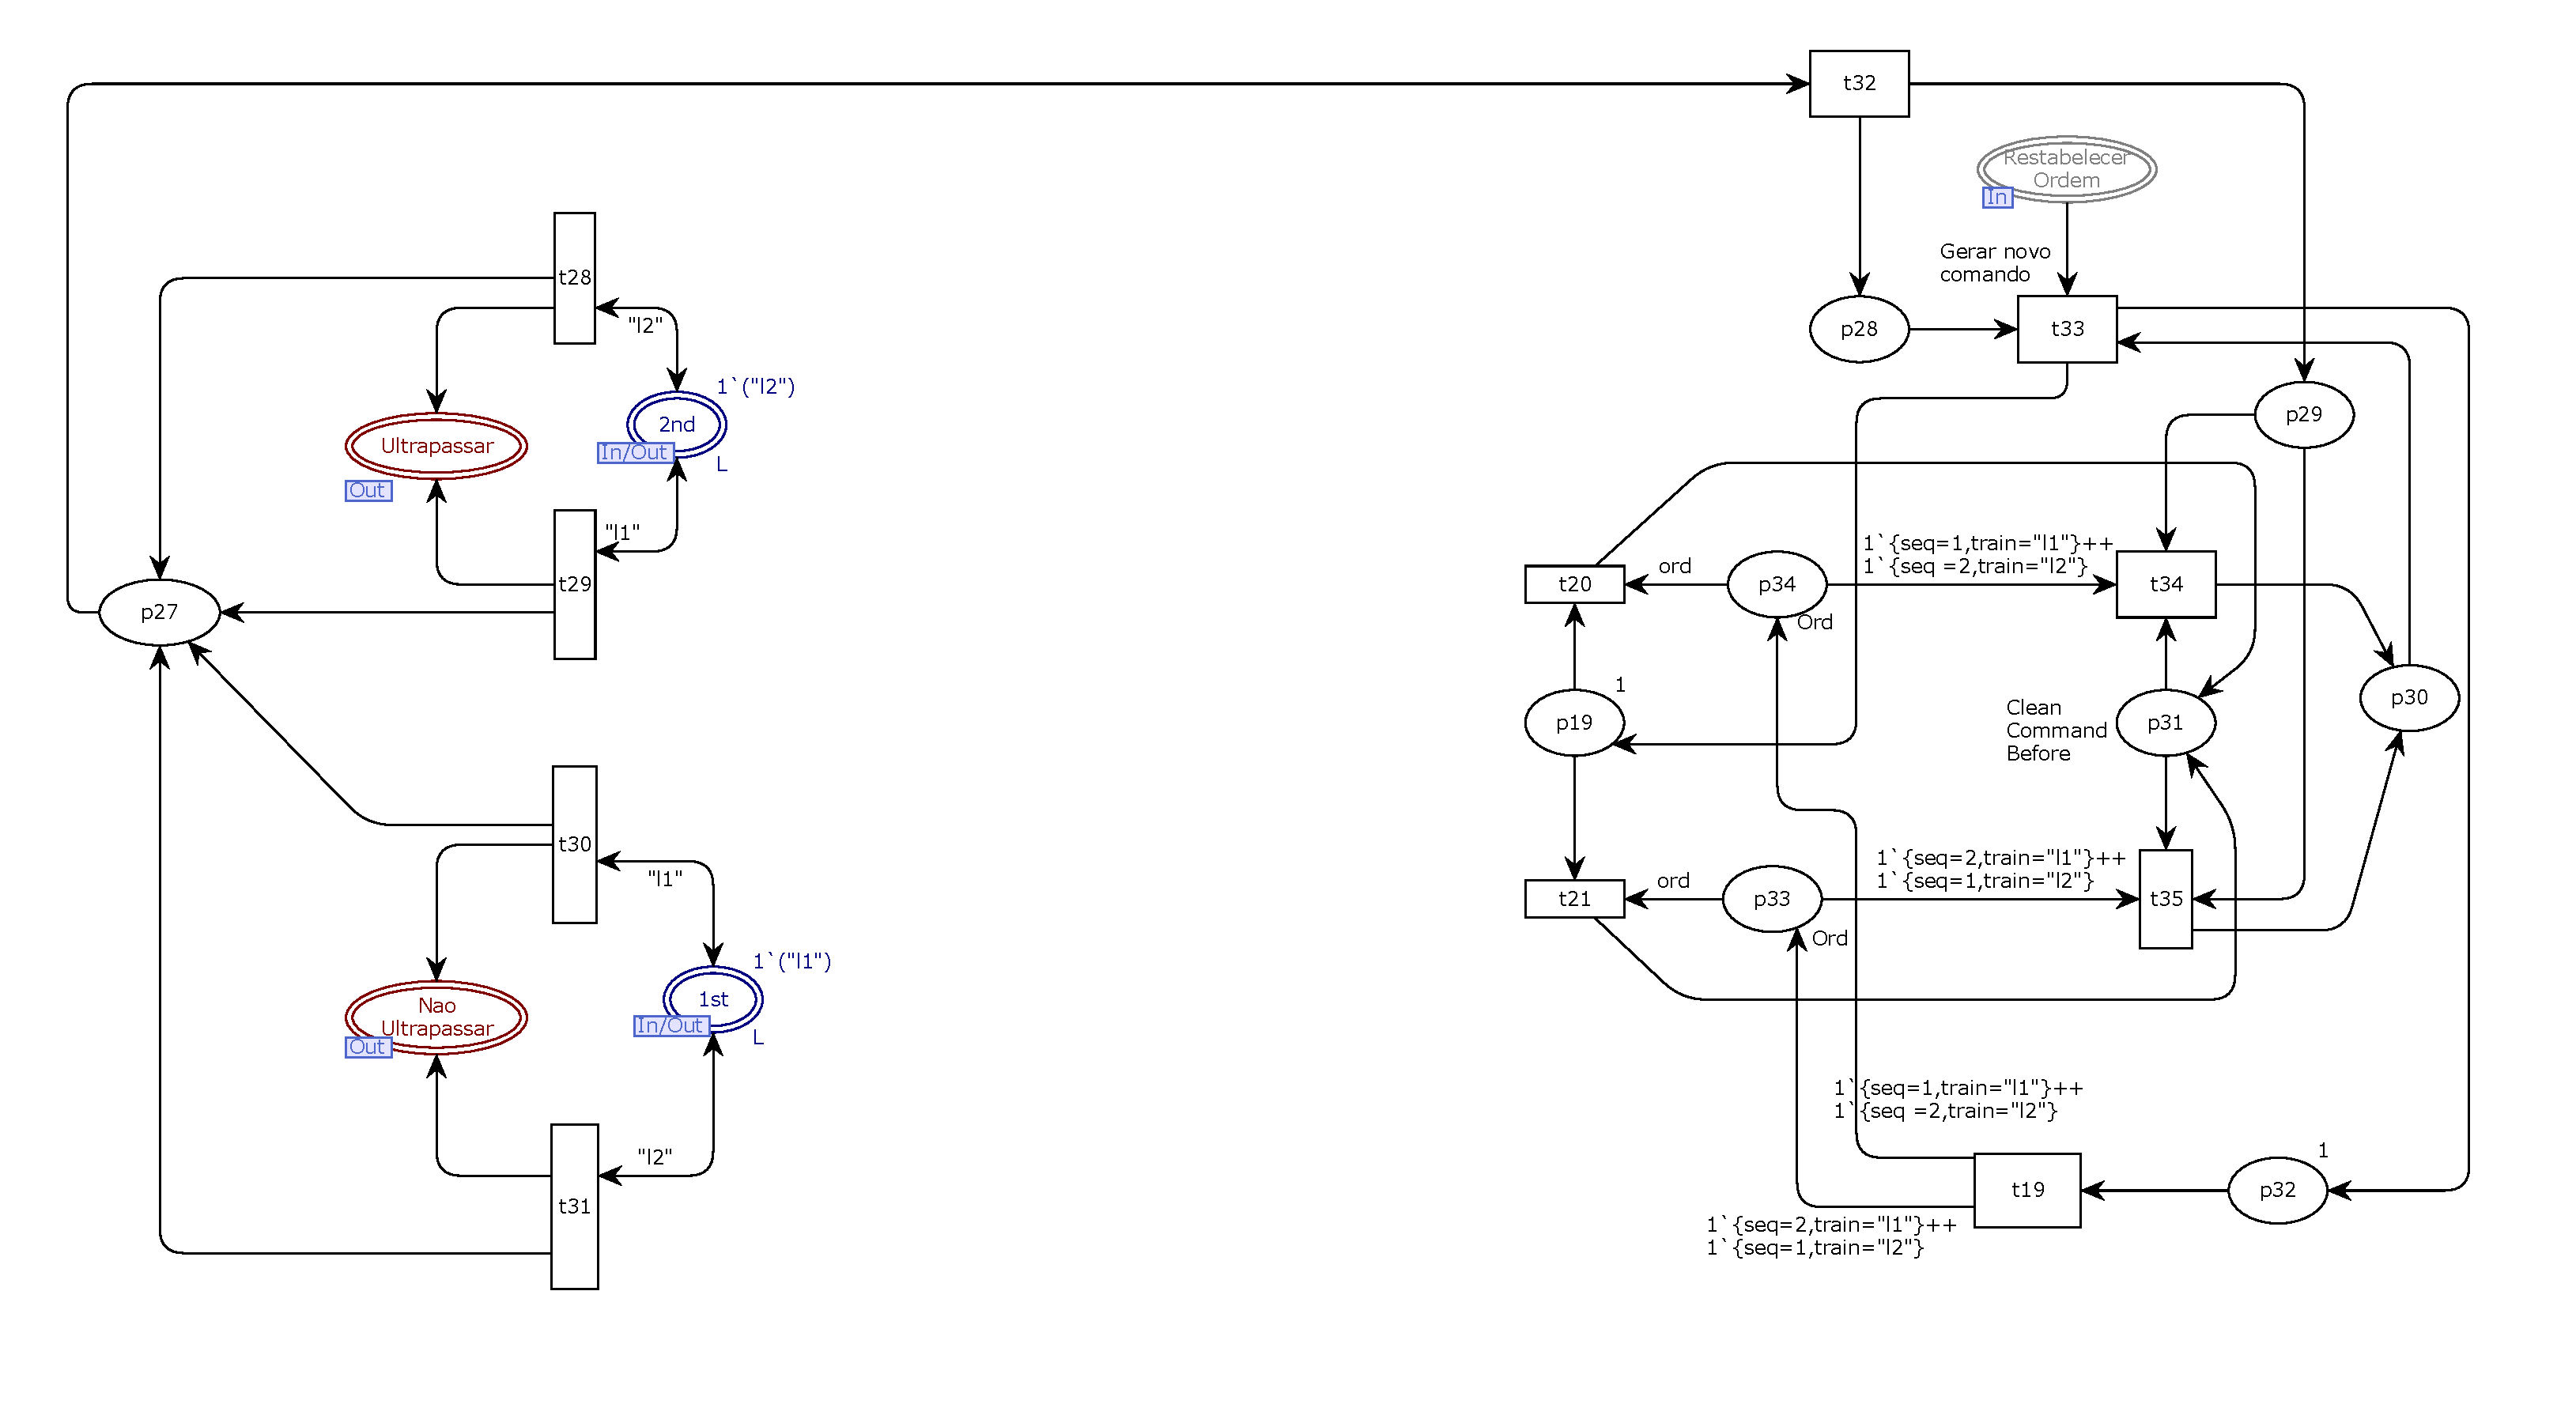
\includegraphics[width=1\linewidth]{figures/Simulation/Modelagem/restabelecer_ordem.eps}
    \legend{Fonte: Elaborado pelo autor.}
\end{figure}

O ultimo componente hierárquico da rede é o de \textit{Inverter Ordem}, responsável por atualizar os lugares de $1_{st}$ e $2_{nd}$, dado pela RPC representada na figura \ref{fig:inverter_ordem}. Note que ao chegar o comando de atualizar ordem caso haja uma ficha em ultrapassar, é ativado a transição $t_{36}$ que tem como objetivo retirar a ficha que estava em $2_{nd}$ guardar temporariamente em $p_{37}$ enquanto a ficha que estava em primeiro lugar é transferida para o segundo lugar e por fim é atualizado o primeiro lugar.
Caso não tenha ocorrido ultrapassagem a transição $t_{37}$ é acionada enviando o comando de \textit{Restabelecer a Rede} para a hierarquia a cima.

\begin{figure}[ht]
    \centering
    \caption{Máscara referente ao restabelecimento do componente de Ordem na RPC}
    \label{fig:inverter_ordem}
    \includegraphics[width=1\linewidth]{figures/Simulation/Modelagem/inverter_ordem.eps}
    \legend{Fonte: Elaborado pelo autor.}
\end{figure}

\section{Controle Cooperativo aplicado a Multiagentes}
Posteriormente à detalhada modelagem do sistema na seção \ref{sec:model_RPC} que foi definida os principais eventos do sistema, além da arquitetura da rede que gera algumas regras para o deslocamento dos vagões é buscada um controle de nível superior responsável por otimizar a referência de posição de cada vagão. Para o desenvolvimento do controle cooperativo entre os vagões com o objetivo de evitar colisões e promover a otimização das trajetórias é importante garantir que as transições na rede de petri possuem acionamentos praticamente instantâneos não influenciando assim de forma significativa na dinâmica do sistema.


